\section{LLM}
\subsection{LLM in Process Mining}
Large Language Models (LLMs) offer powerful capabilities for enhancing process mining tasks, particularly in the realm of data augmentation. Data augmentation refers to the practice of expanding or enriching datasets by generating new, synthetic, or modified data samples while maintaining the underlying structure and semantics of the original dataset. This is especially valuable in process mining, where real-world event logs may be sparse, incomplete, or lack variability.

In the context of process mining, LLMs can be employed to:
\begin{itemize}
    \item \textbf{Generate Synthetic Event Logs:} LLMs can create realistic sequences of events that simulate user or system behaviors, adhering to predefined process constraints.
    \item \textbf{Enhance Incomplete Logs:} Missing events or timestamps in logs can be filled in a coherent manner, ensuring that the augmented data aligns with the actual process flows.
    \item \textbf{Introduce Controlled Variability:} By simulating alternative pathways or deviations within a process, LLMs can produce diverse scenarios, aiding in stress-testing and robustness analysis of process models.
\end{itemize}

The use of LLMs for data augmentation not only improves the quality and quantity of datasets but also enables better model training.
In this study, data augmentation was performed using:
\begin{itemize}
    \item \textbf{GPT-4o:} A state-of-the-art LLM developed by OpenAI
    \item \textbf{Mistral:} An LLM developed in France
    \item \textbf{Gemini 2.0 Flash Experimental}: The last version of the Gemini model, developed by Google
\end{itemize}
All 3 LLMs were given the following promp
\textit{Perform a data augmentation task on this dataset, creating new consistent data} with the original dataset attached
\subsection{Experiment performed}
\subsubsection{GPT-4o}
The GPT-4o returned only 60 new events, a number of new events significantly lower than expected. The model seemed to struggle with the complexity of the process and the constraints imposed by the dataset. Here the results:

\begin{figure}[H]
    \centering
    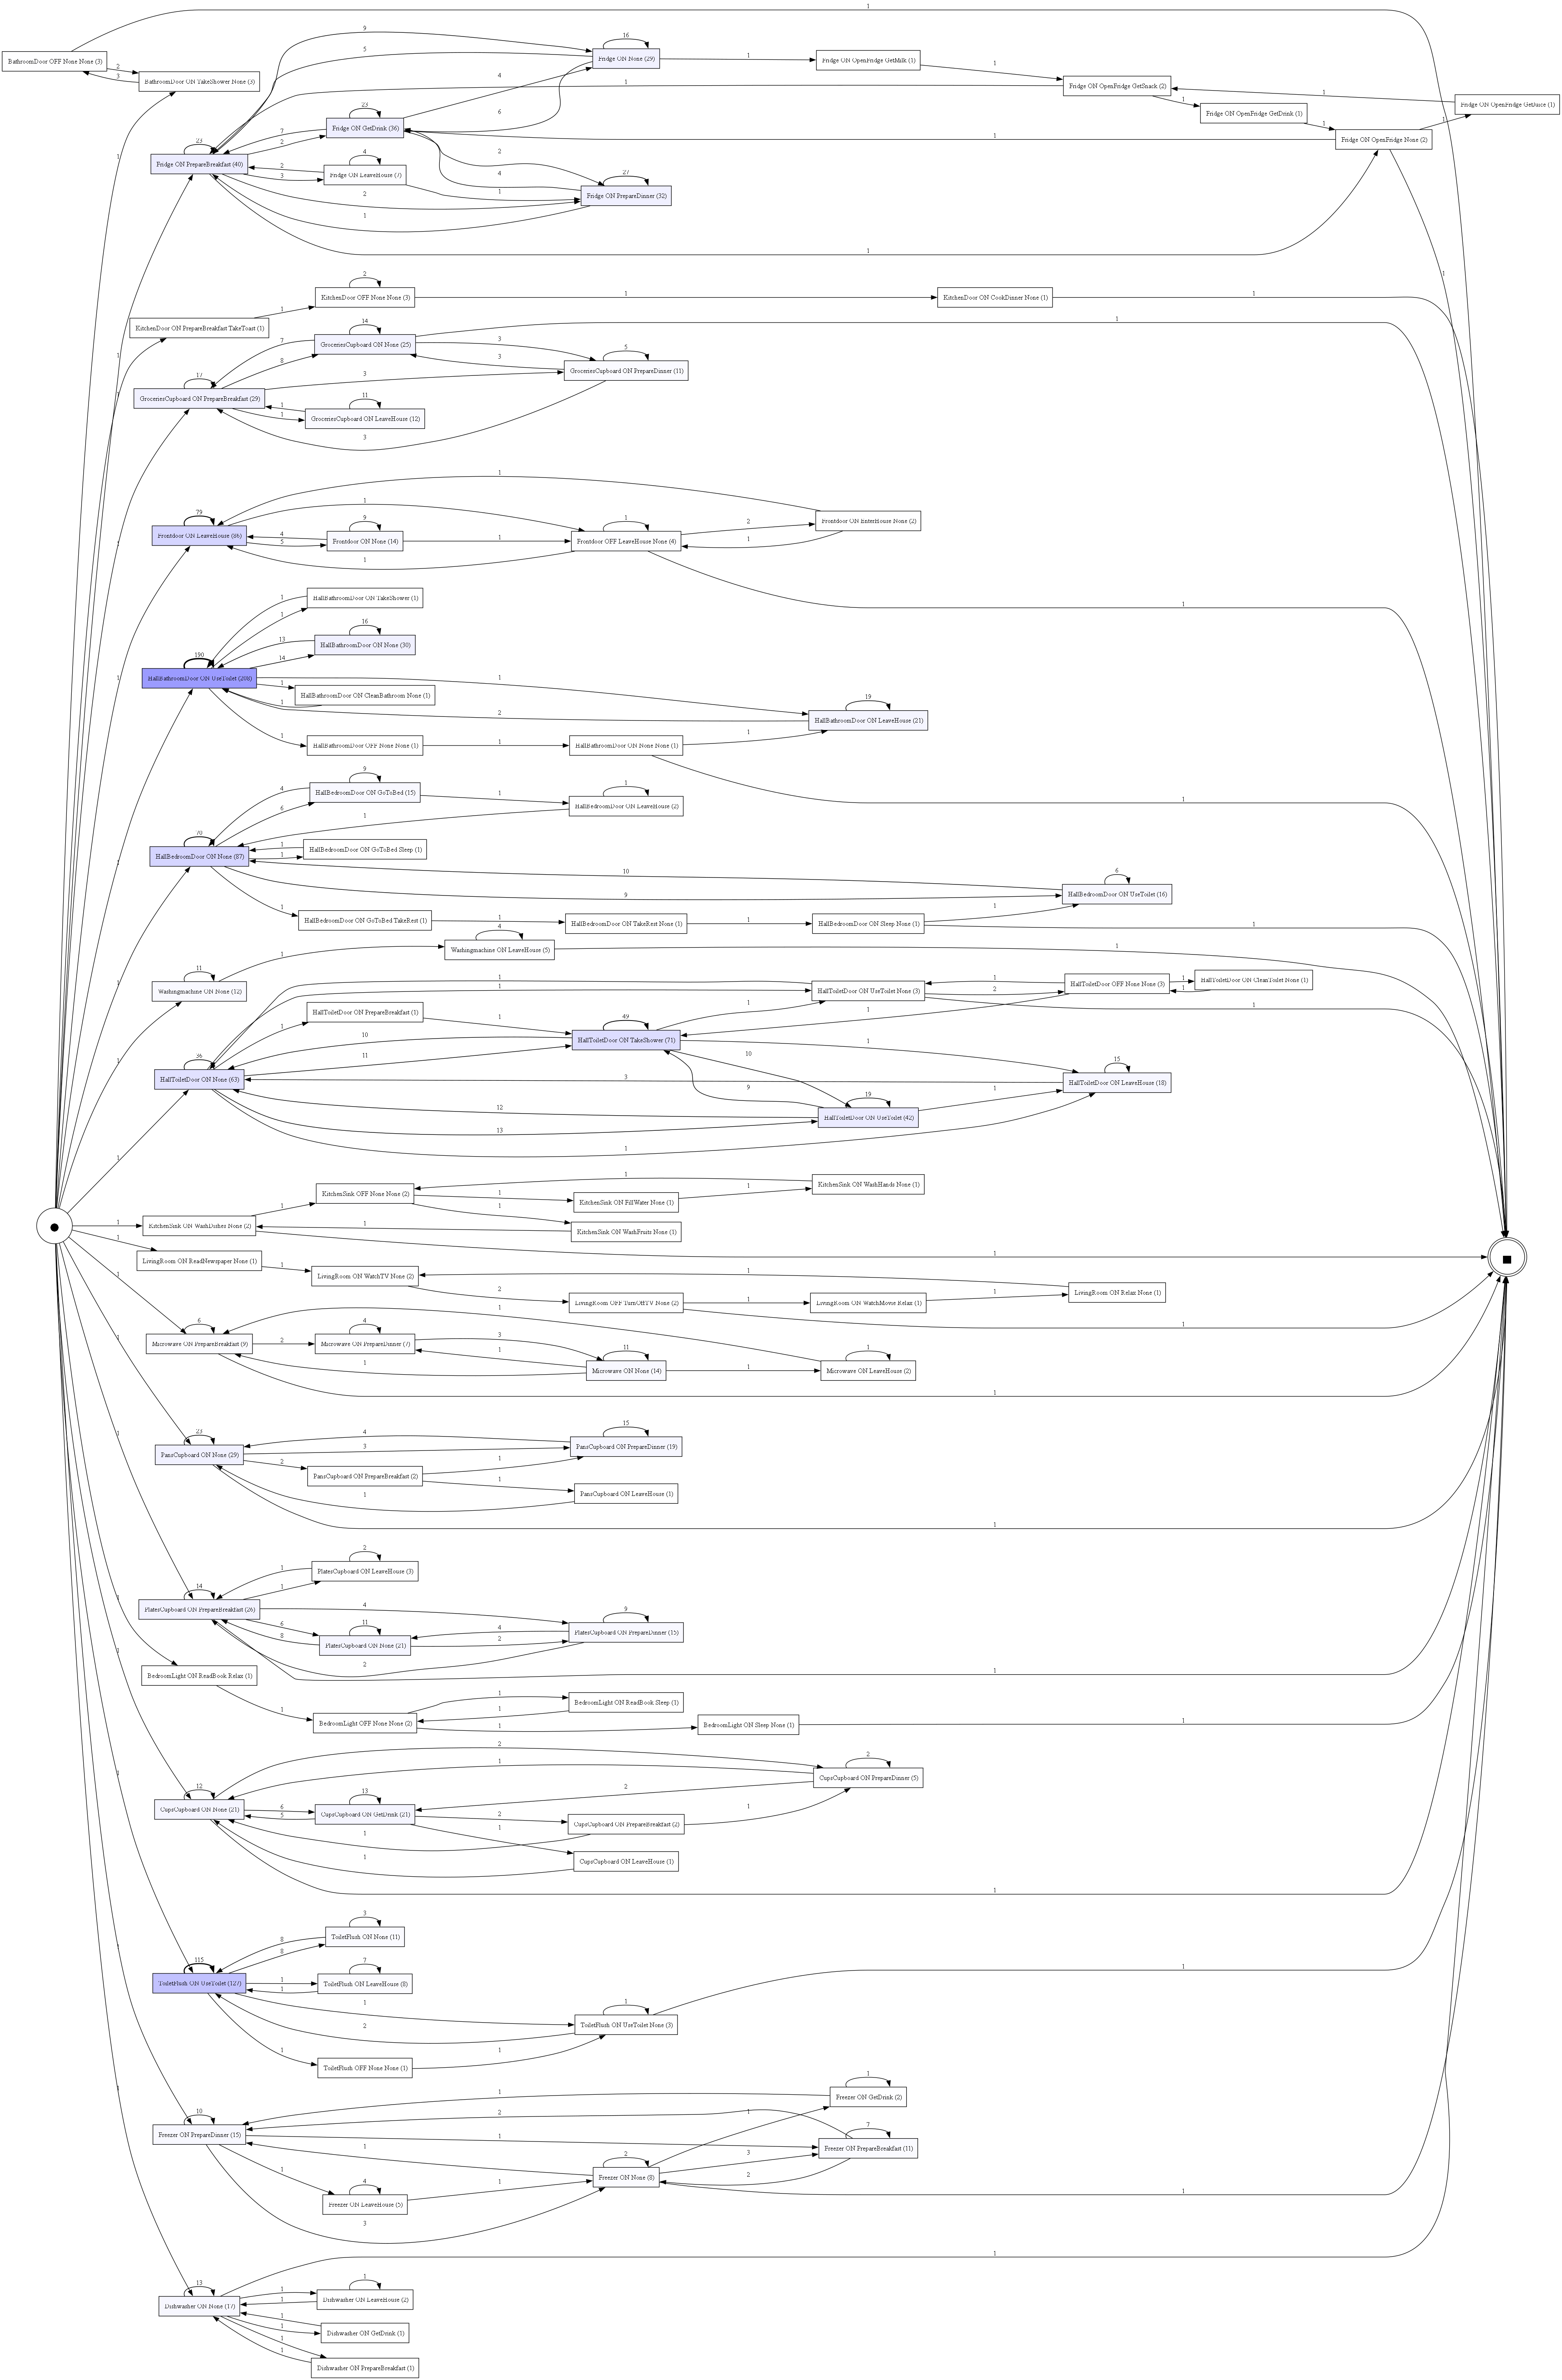
\includegraphics[width=\linewidth, height=\textheight]{images/dfgGPT.png}
    \caption{Directly-Follows Graph (DFG) of the event log}
\end{figure}

\begin{figure}[H]
    \centering
    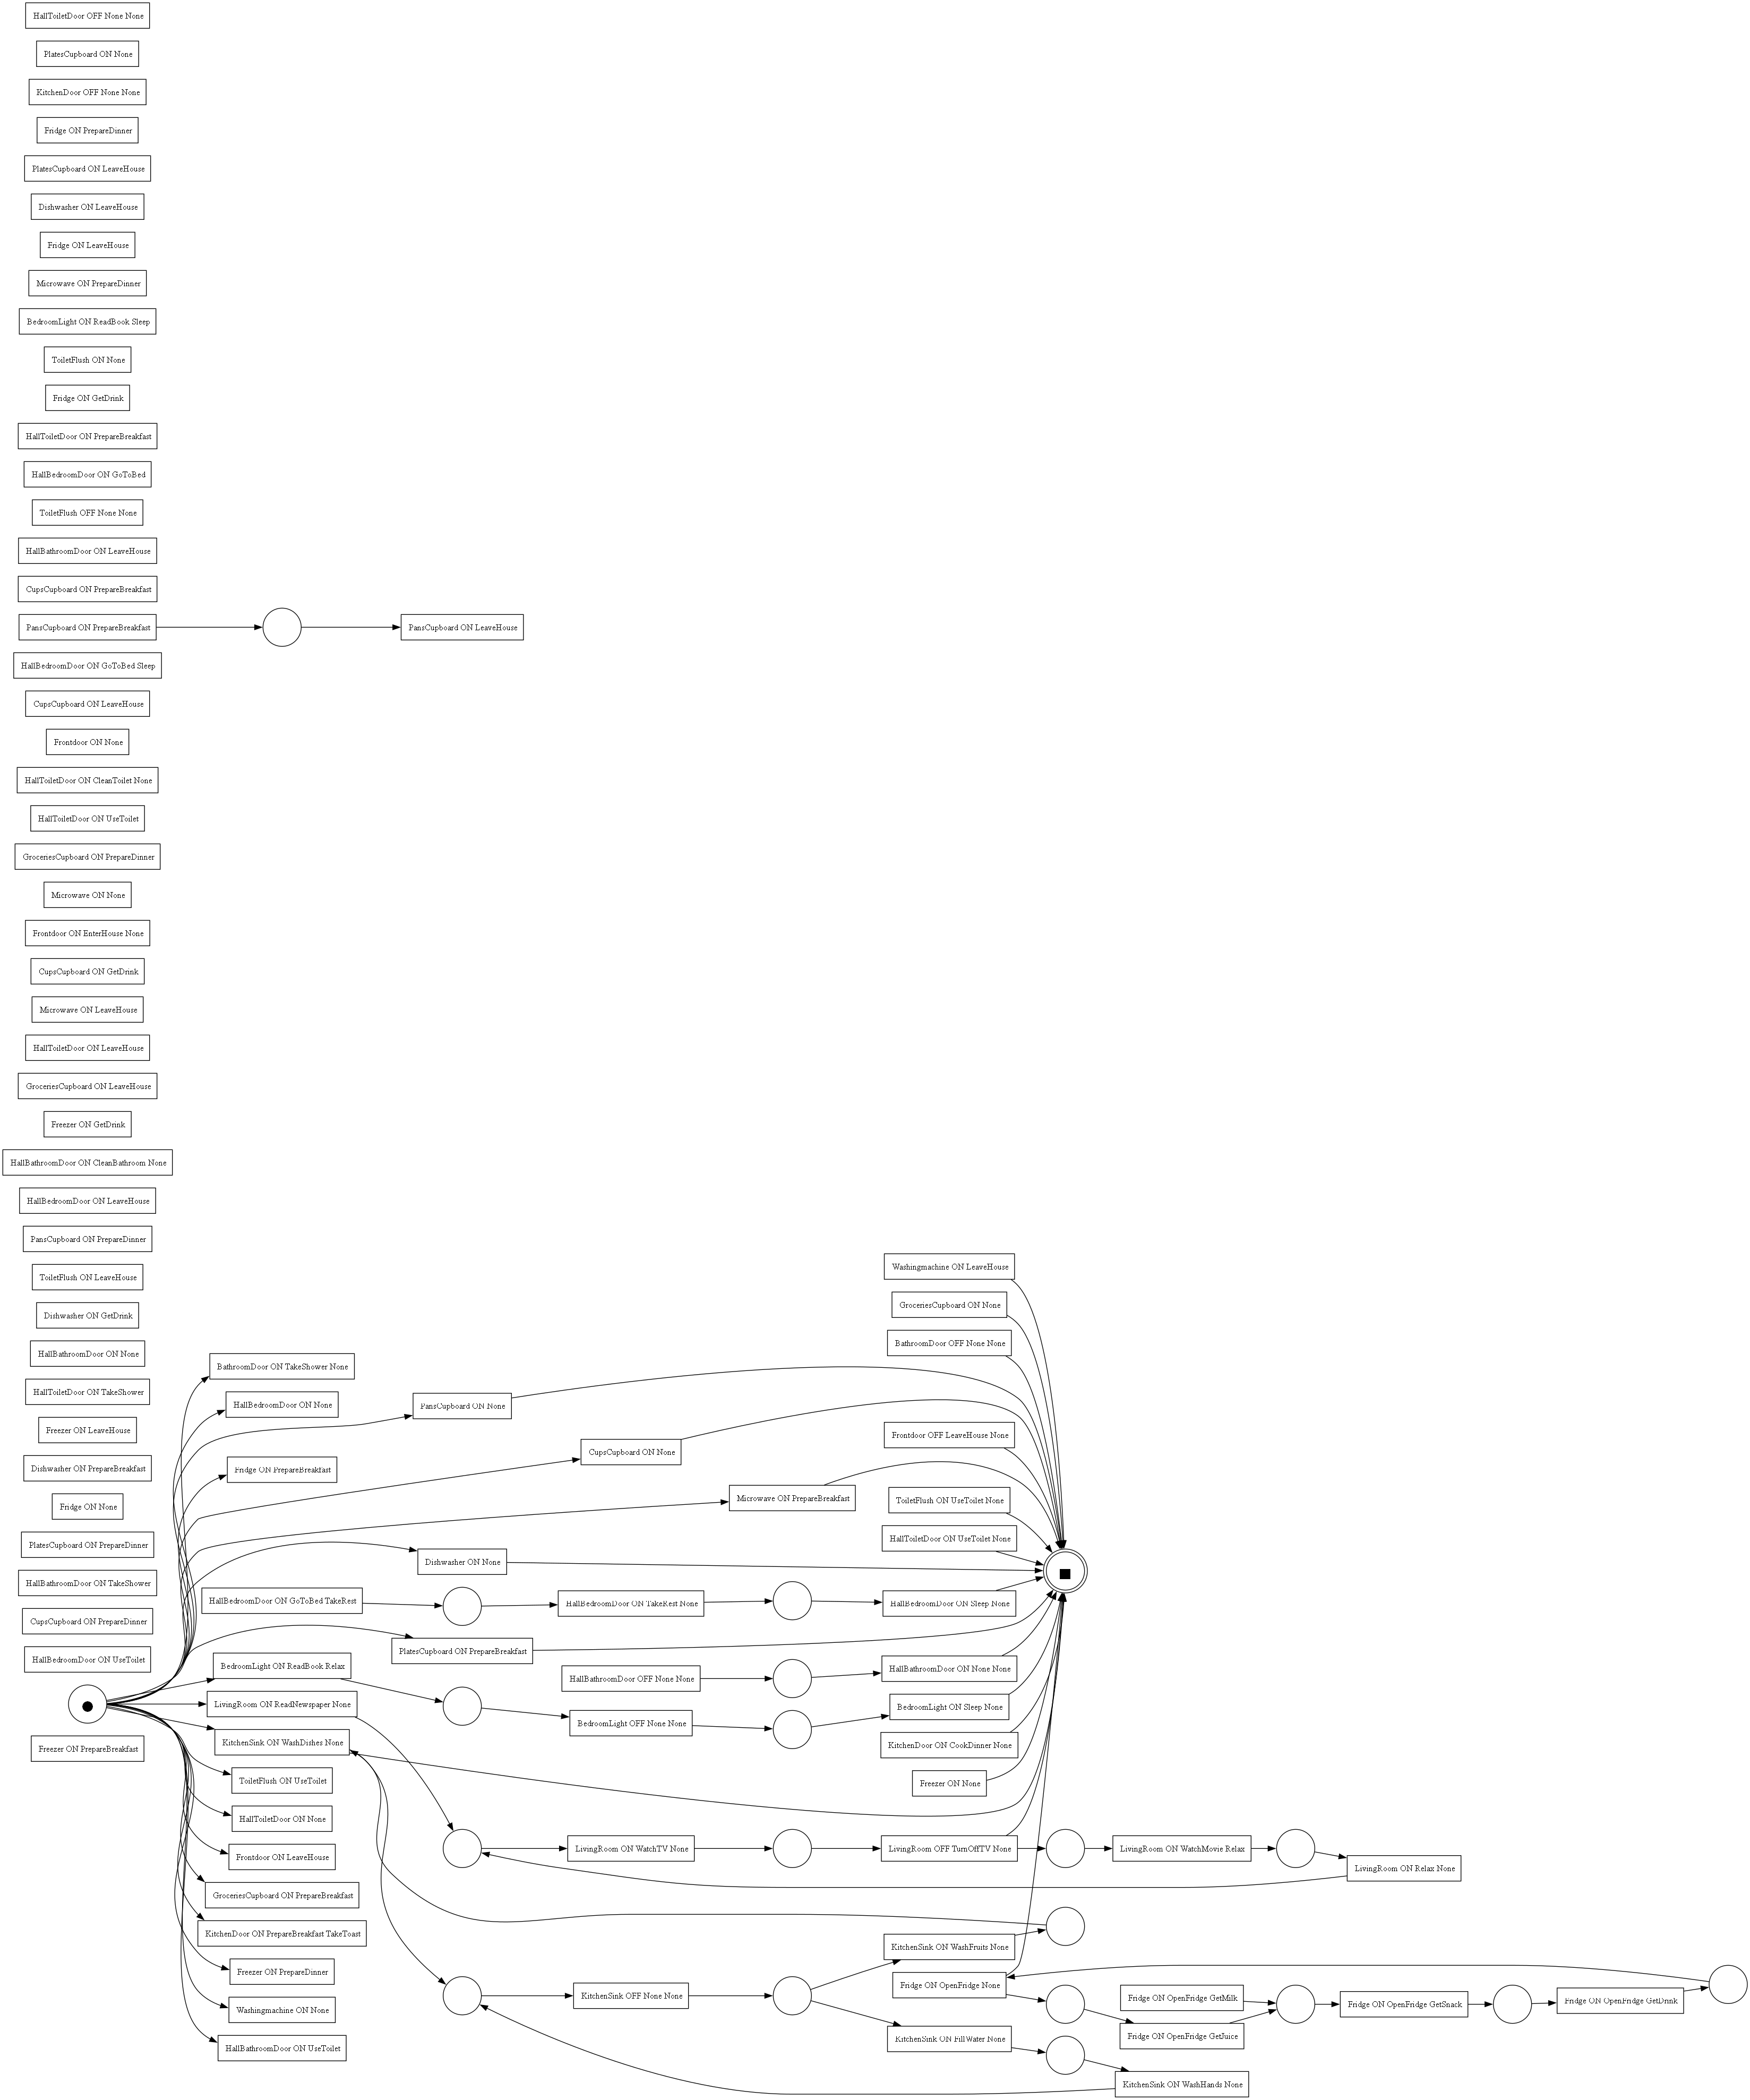
\includegraphics[width=\linewidth, height=\textheight]{images/alpha_minerGPT.png}
    \caption{Alpha Miner Petri Net}
\end{figure}

\begin{figure}[H]
    \centering
    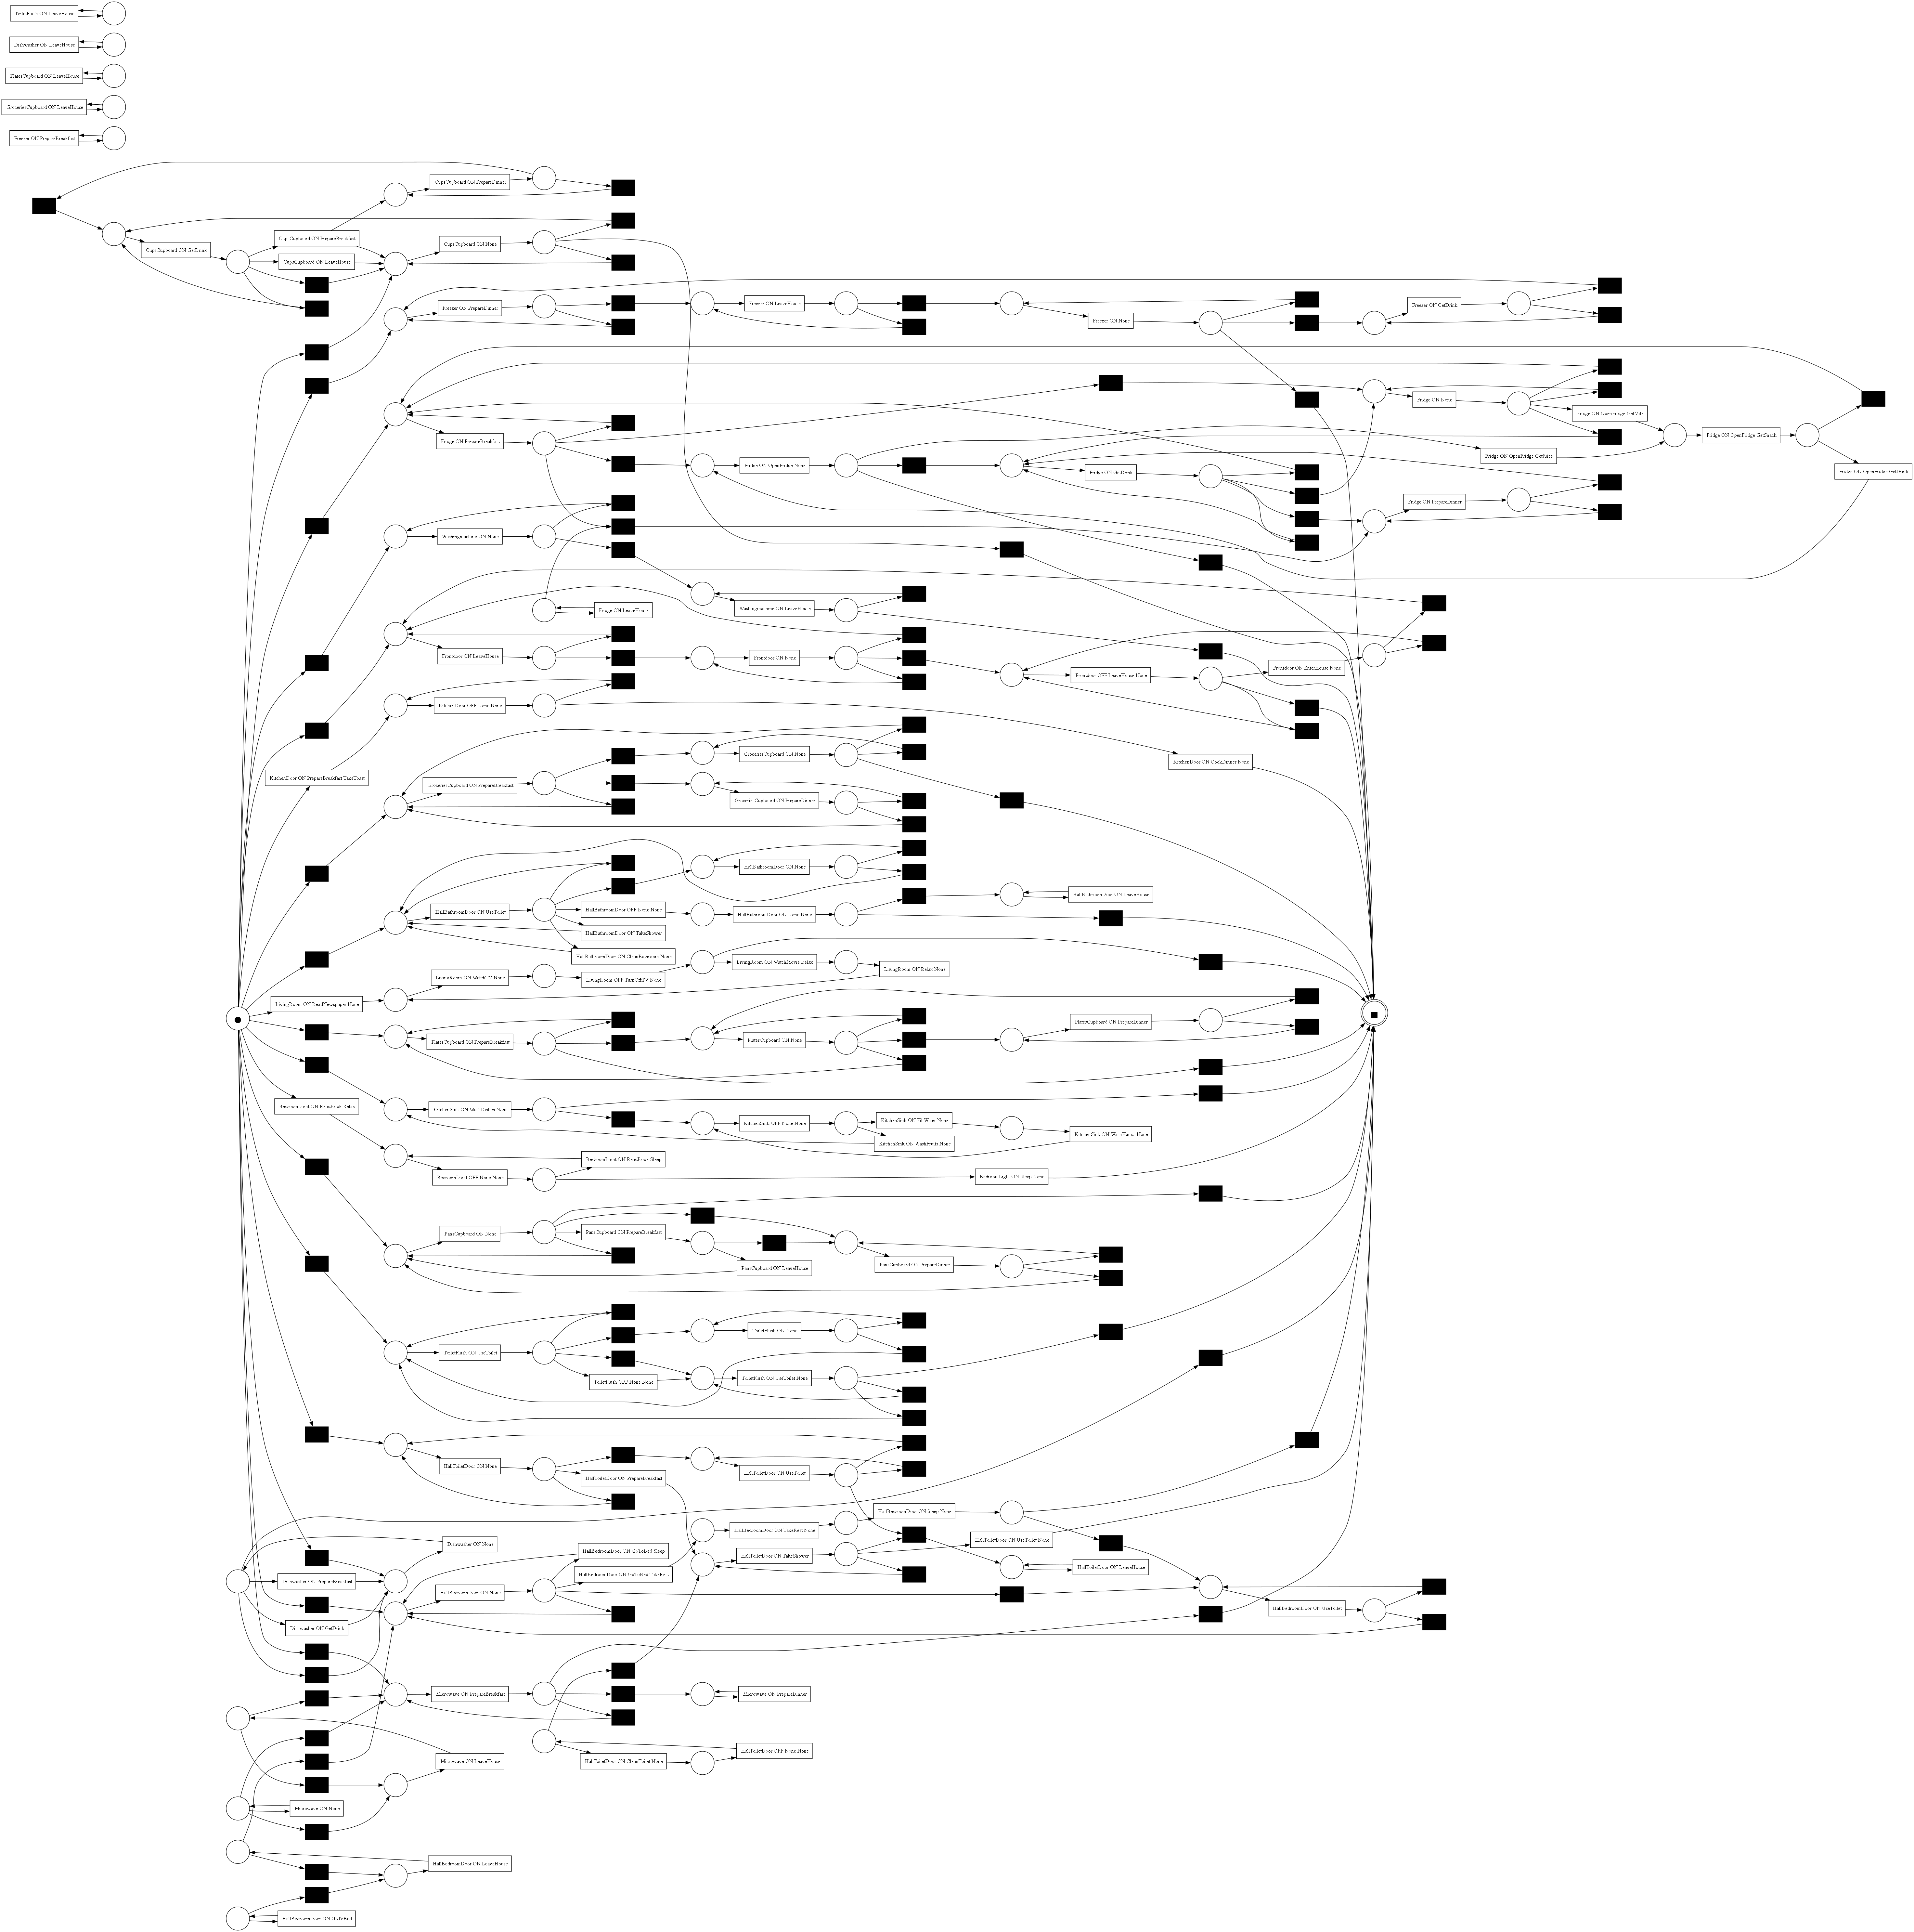
\includegraphics[width=\linewidth, height=\textheight]{images/heuristic_minerGPT.png}
    \caption{Heuristic Miner Petri Net}
\end{figure}

\begin{figure}[H]
    \centering
    \includegraphics[width=\linewidth, height=\textheight]{images/inductive_minerGPT.png}
    \caption{Inductive Miner Petri Net}
\end{figure}



\begin{figure}[H]
    \centering
    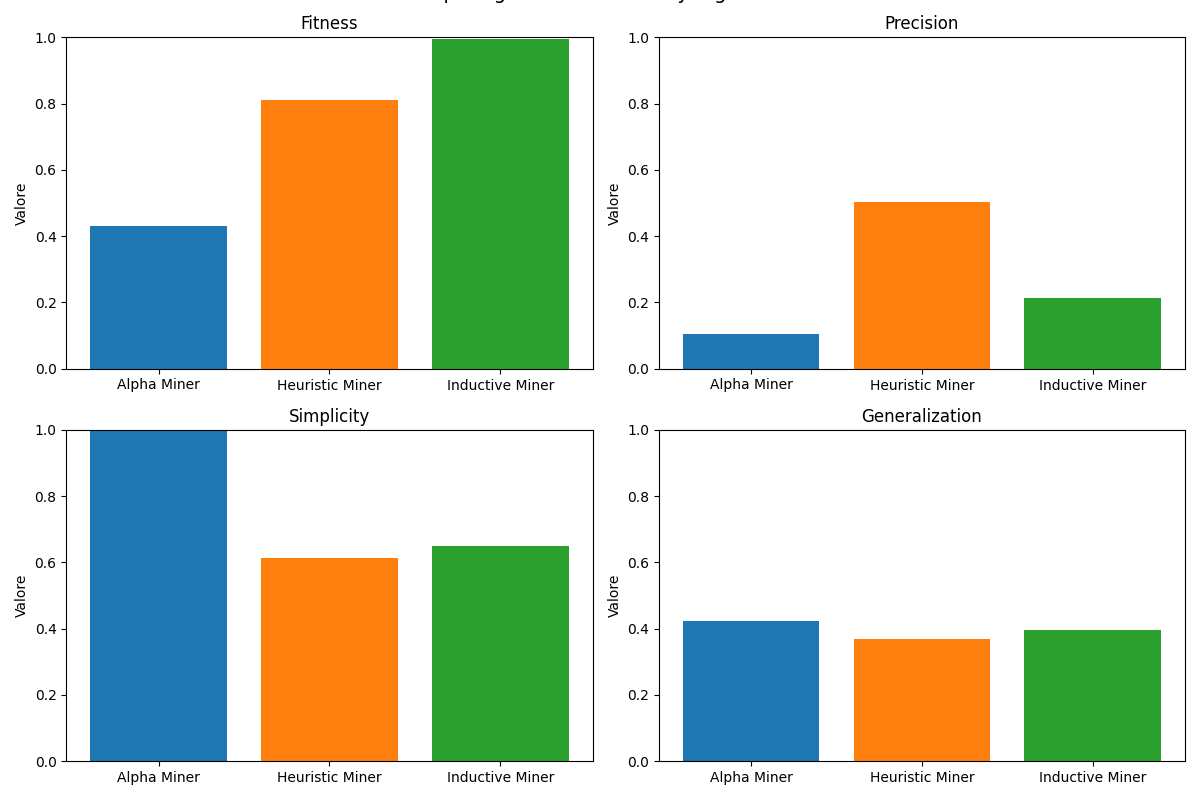
\includegraphics[scale=0.5]{images/metricsGPT.png}
    \caption{Performance metrics of the process mining algorithms}
\end{figure}


\begin{itemize}
    \item \textbf{Fitness:} Slightly reduced for all the algorithms
    \item \textbf{Precision:} Improves for Heuristic Miner, Reduced for Inductive Miner
    \item \textbf{Simplicity:} Same results
    \item \textbf{Generalization:} Reduced for all the algorithms
\end{itemize}

\subsubsection{Gemini 2.0 Flash Experimental}
The Gemini 2.0 Flash Experimental model returned 292 new events: the model was able to generate a more diverse set of sequences compared to GPT-4o. The results are as follows:
\begin{figure}[H]
    \centering
    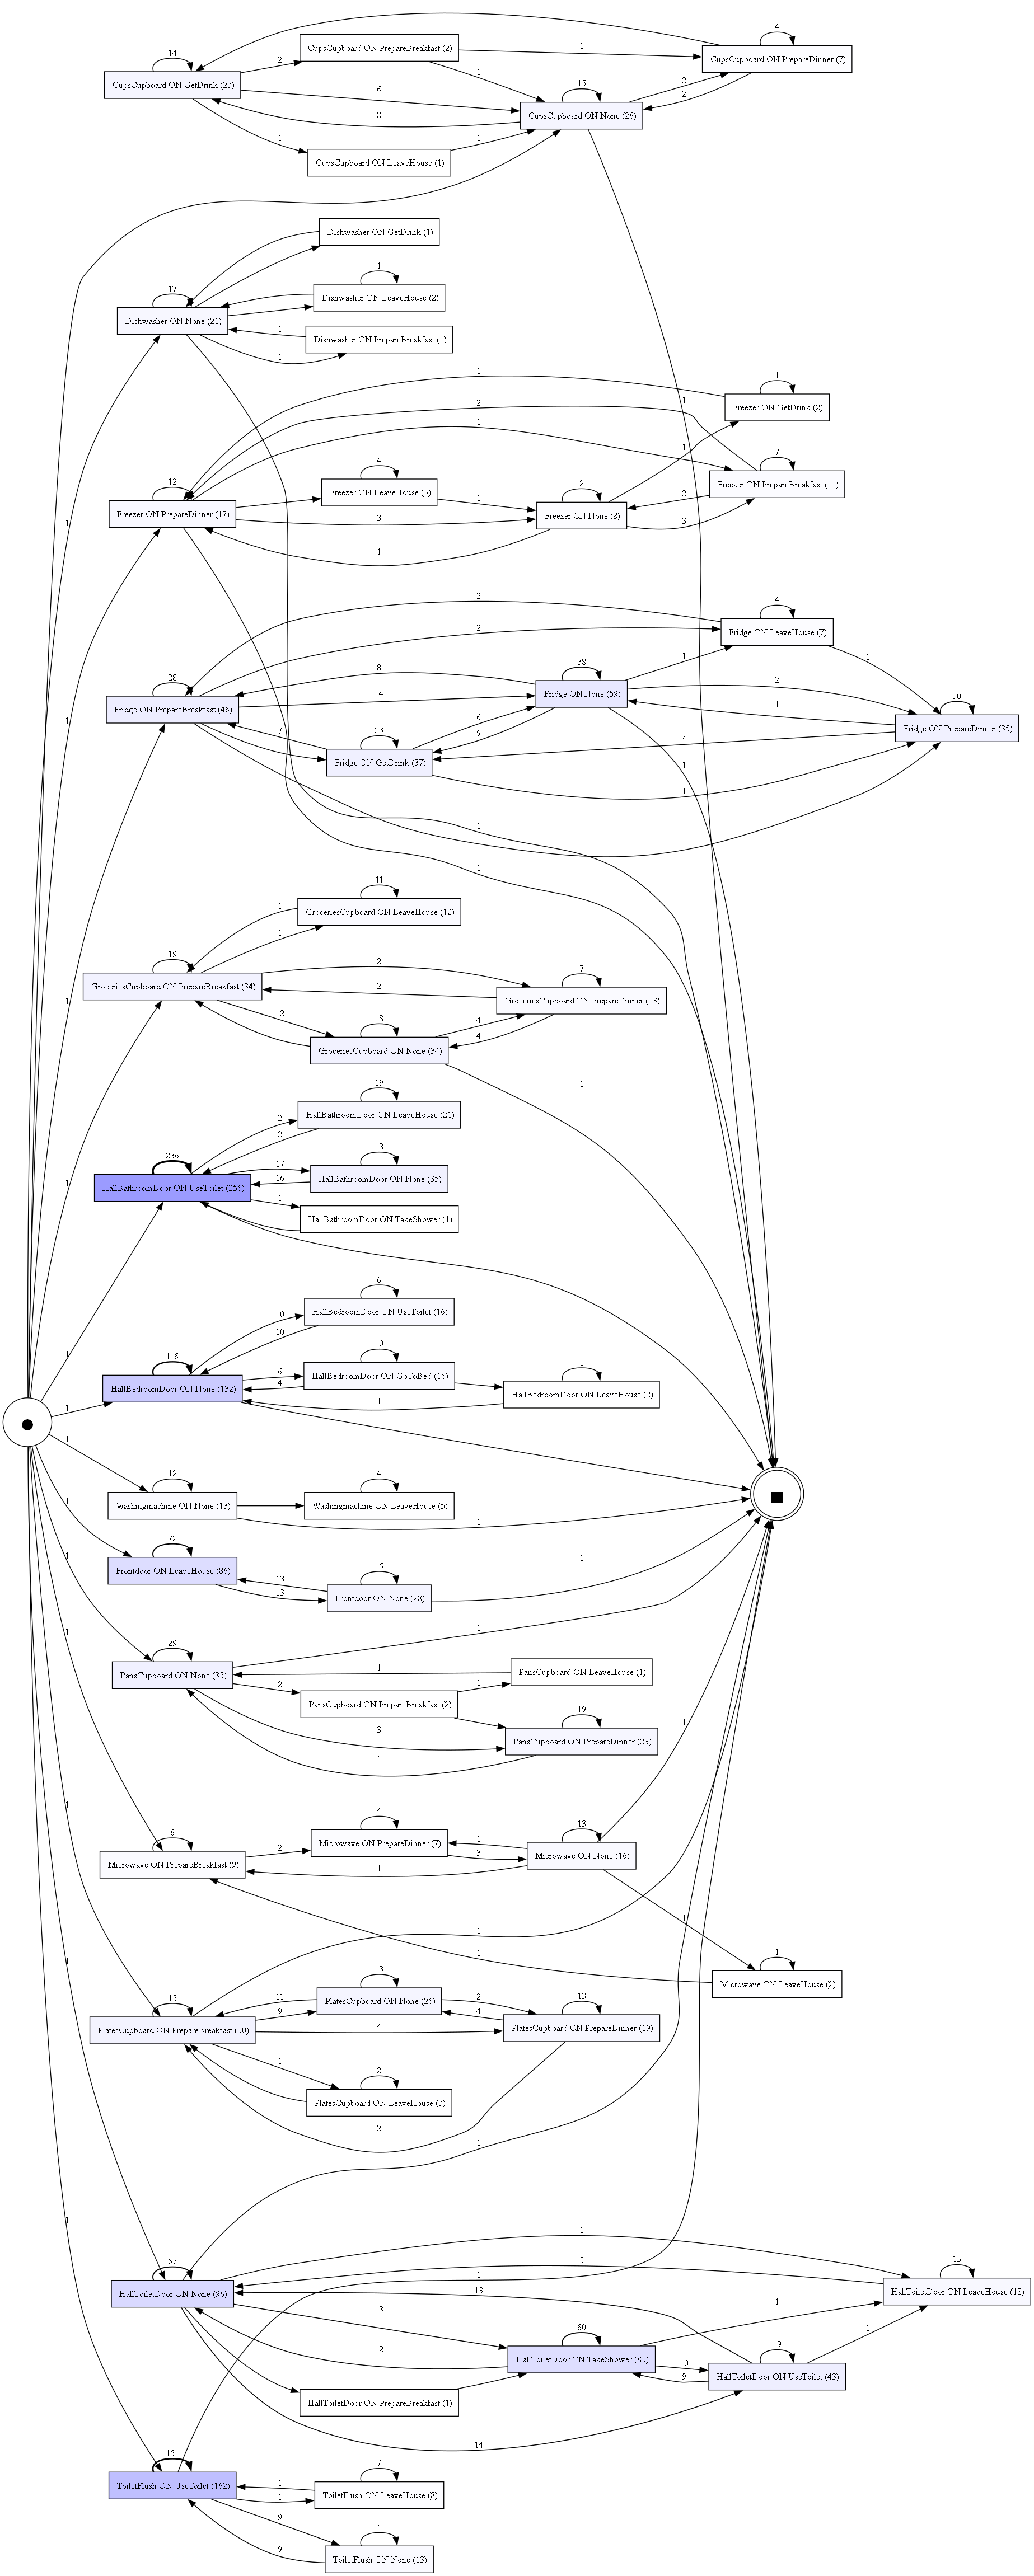
\includegraphics[width=\linewidth, height=\textheight]{images/dfgGemini.png}
    \caption{Directly-Follows Graph (DFG) of the event log}
\end{figure}

\begin{figure}[H]
    \centering
    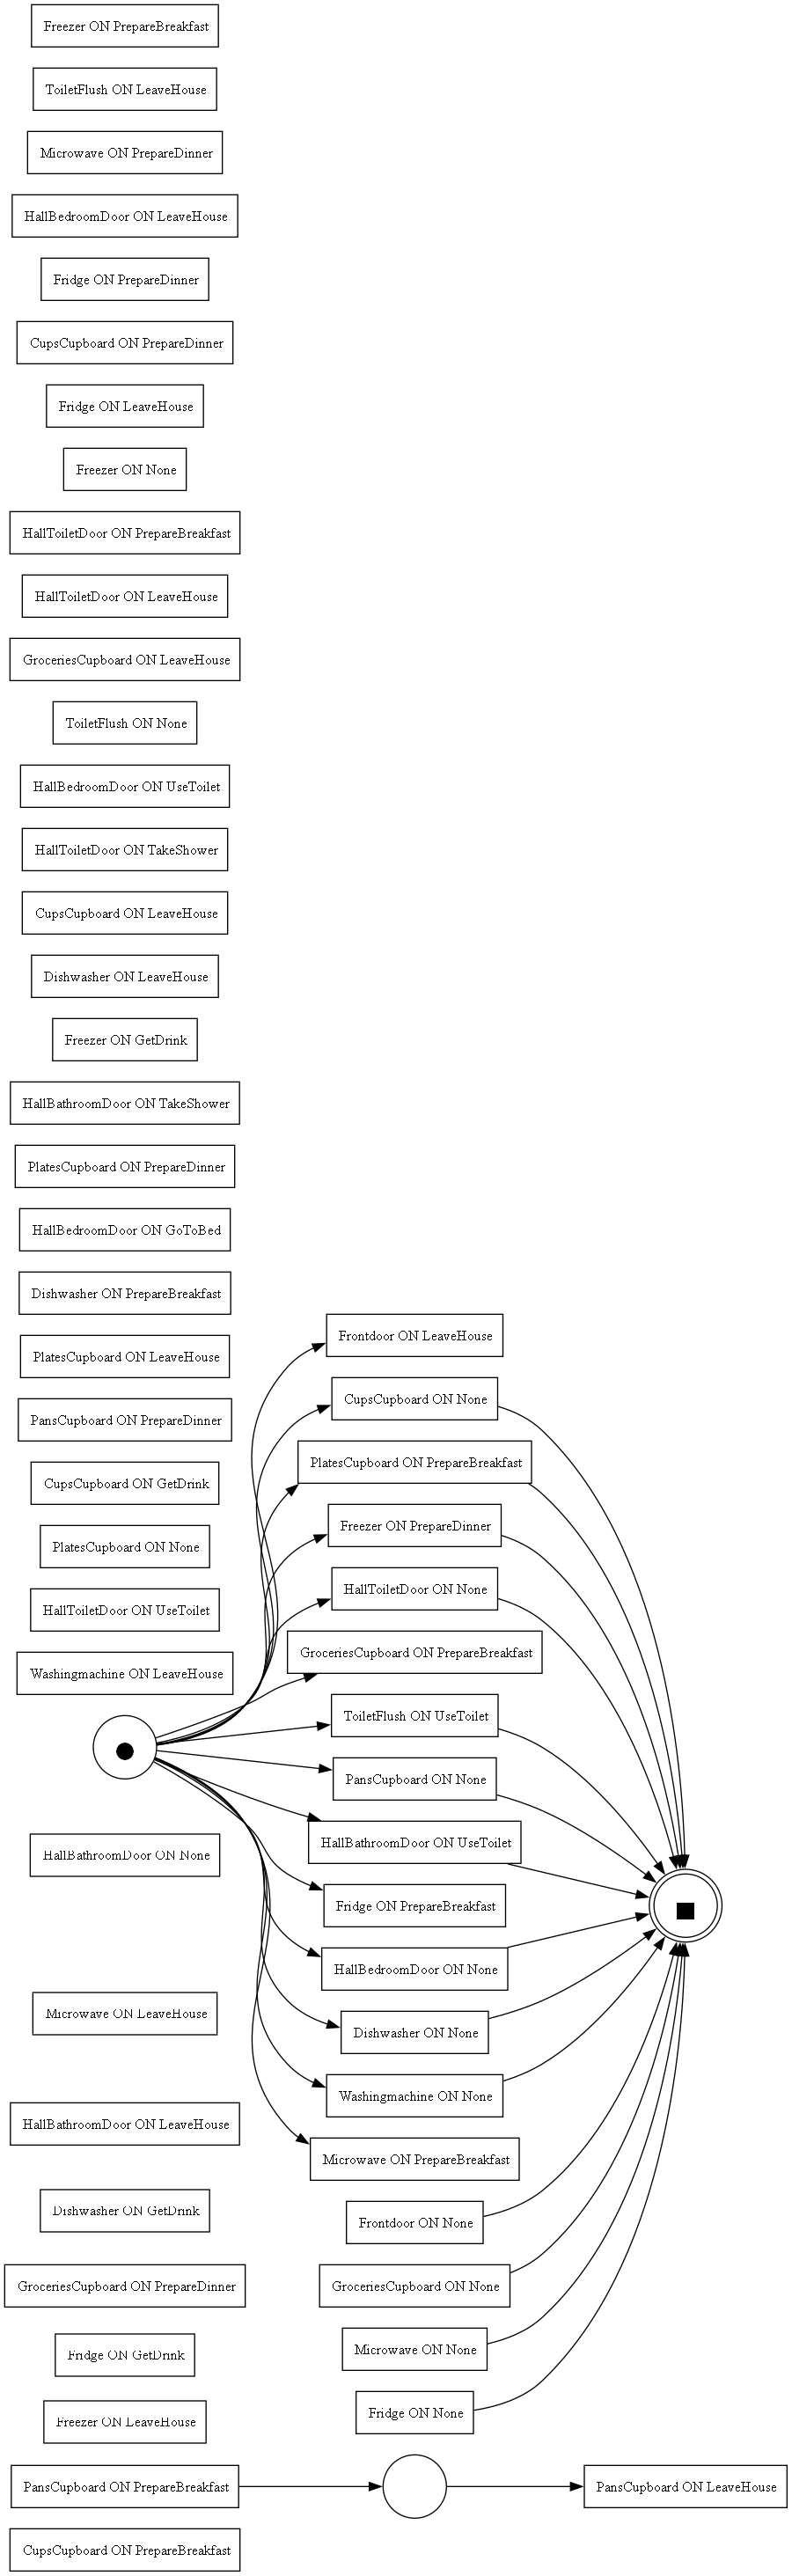
\includegraphics[width=\linewidth, height=\textheight]{images/alpha_minerGemini.png}
    \caption{Alpha Miner Petri Net}
\end{figure}

\begin{figure}[H]
    \centering
    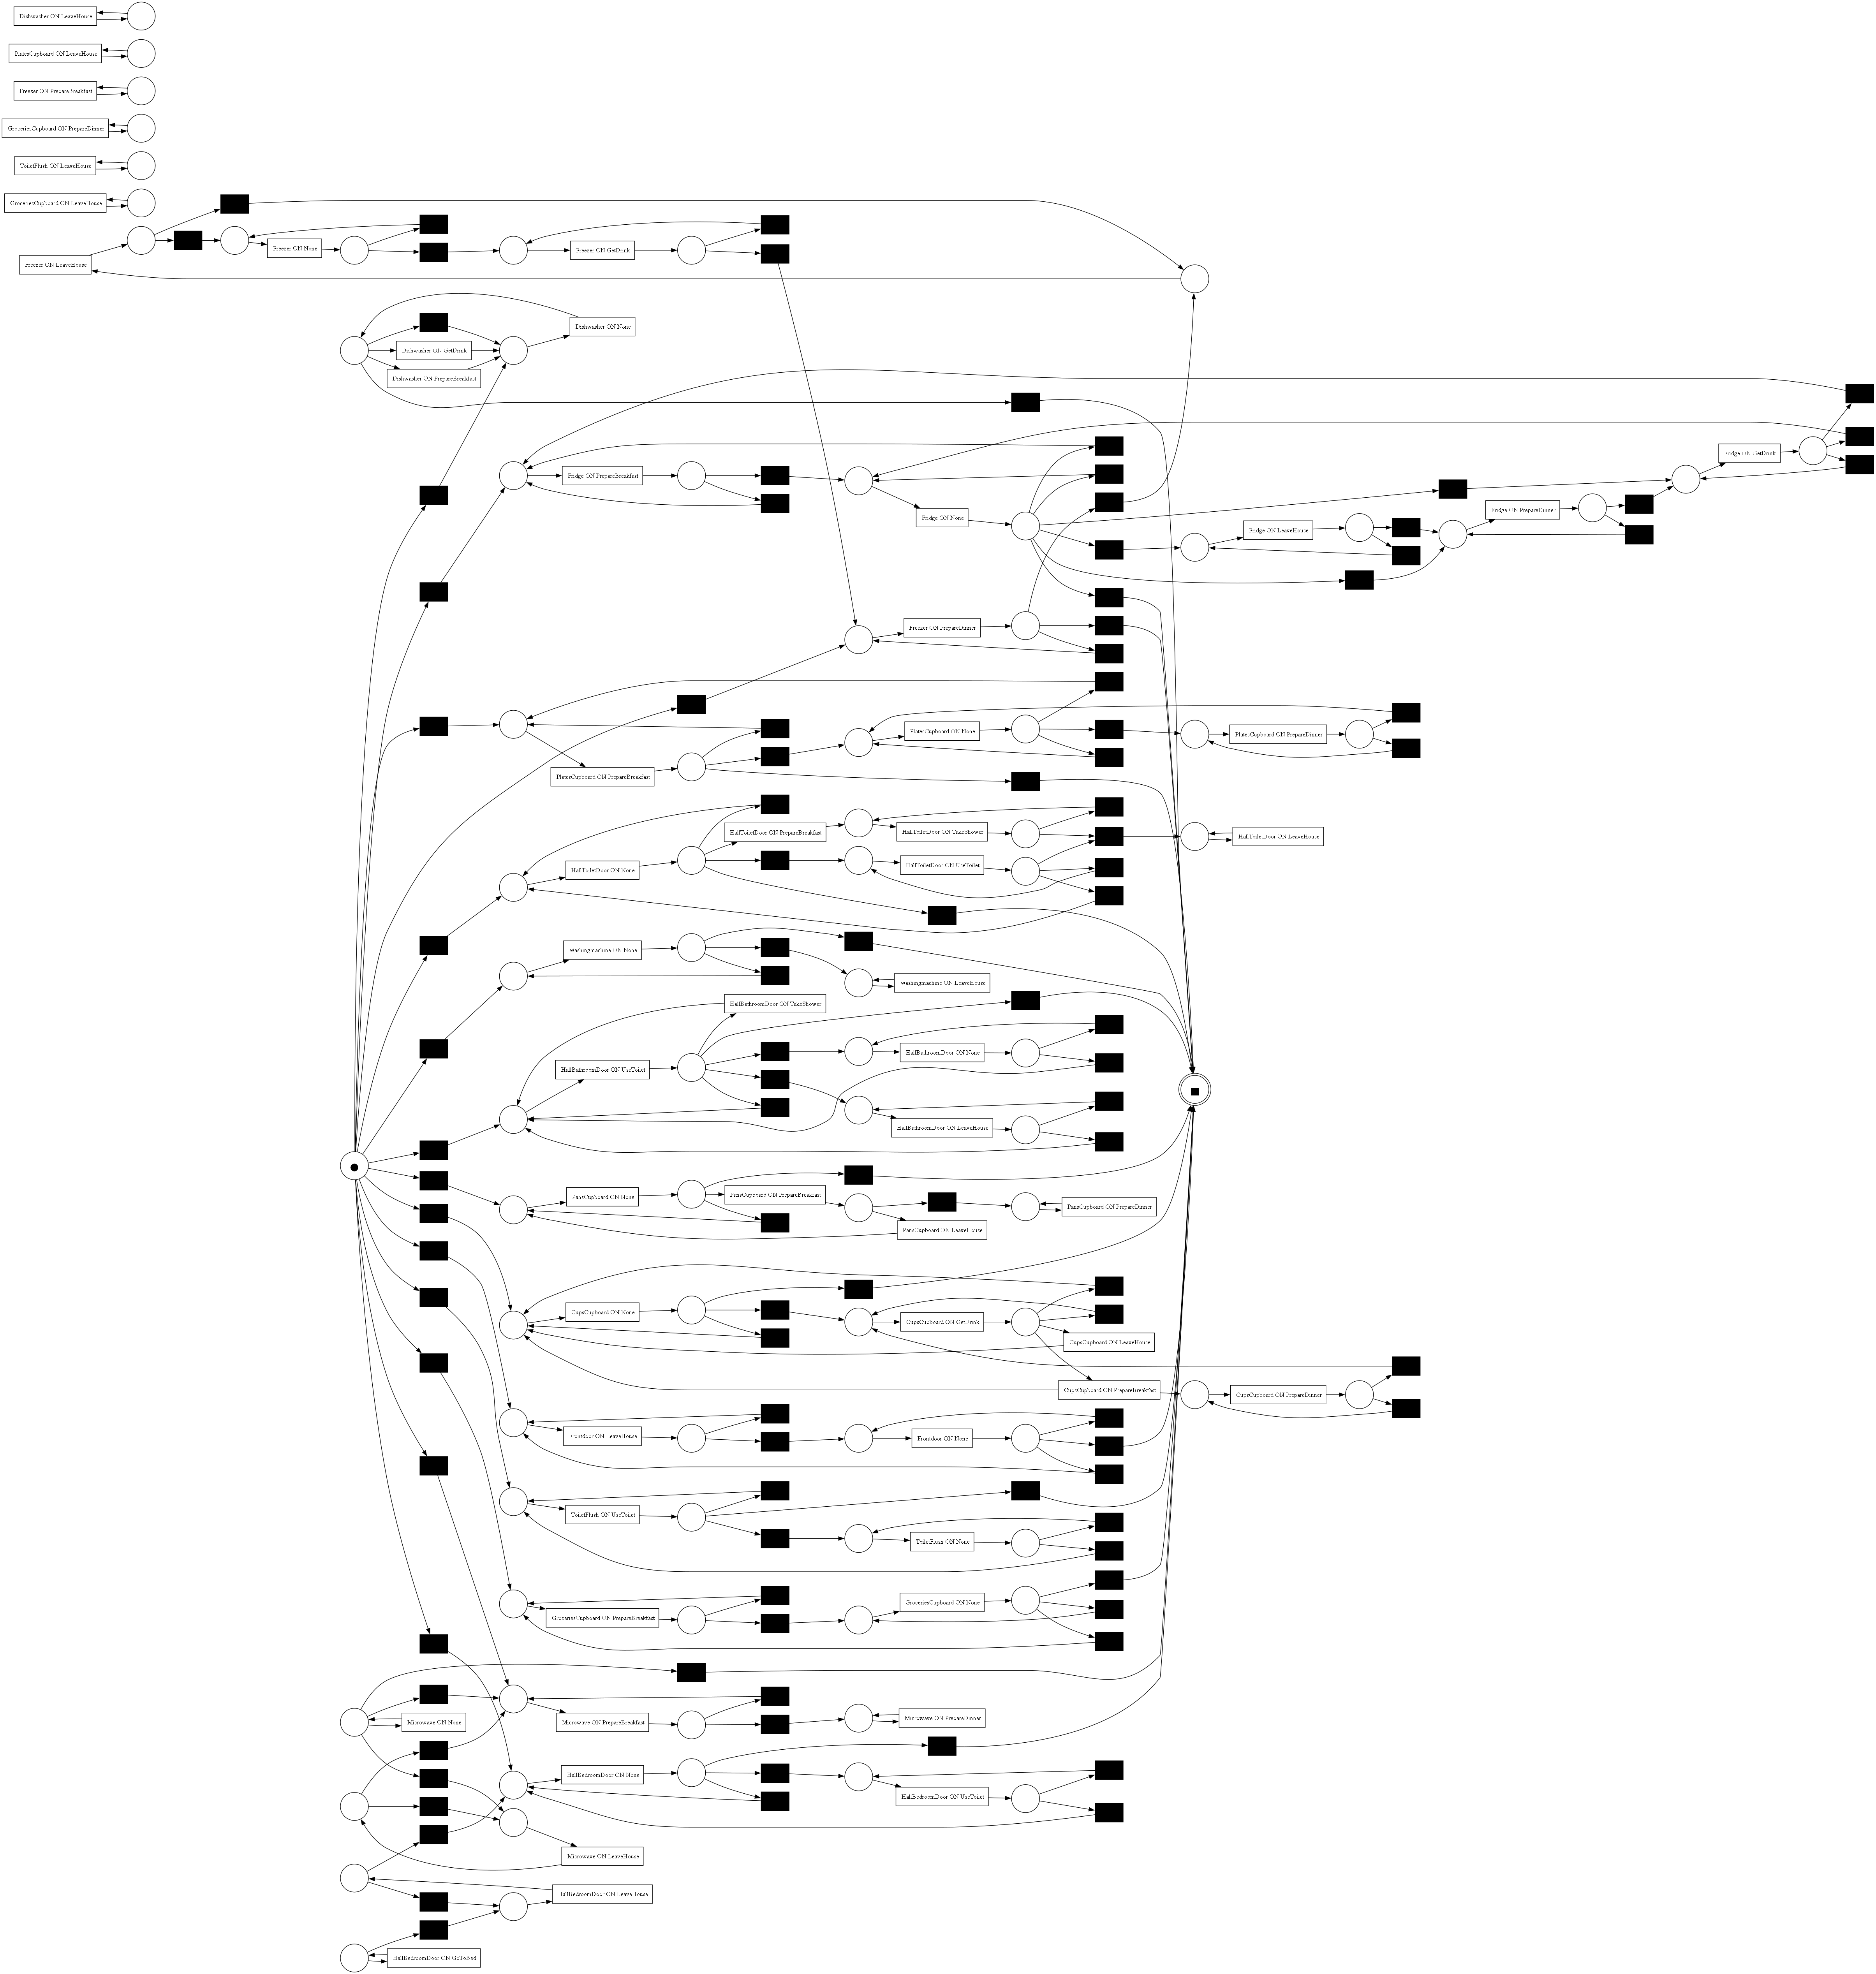
\includegraphics[width=\linewidth, height=\textheight]{images/heuristic_minerGemini.png}
    \caption{Heuristic Miner Petri Net}
\end{figure}

\begin{figure}[H]
    \centering
    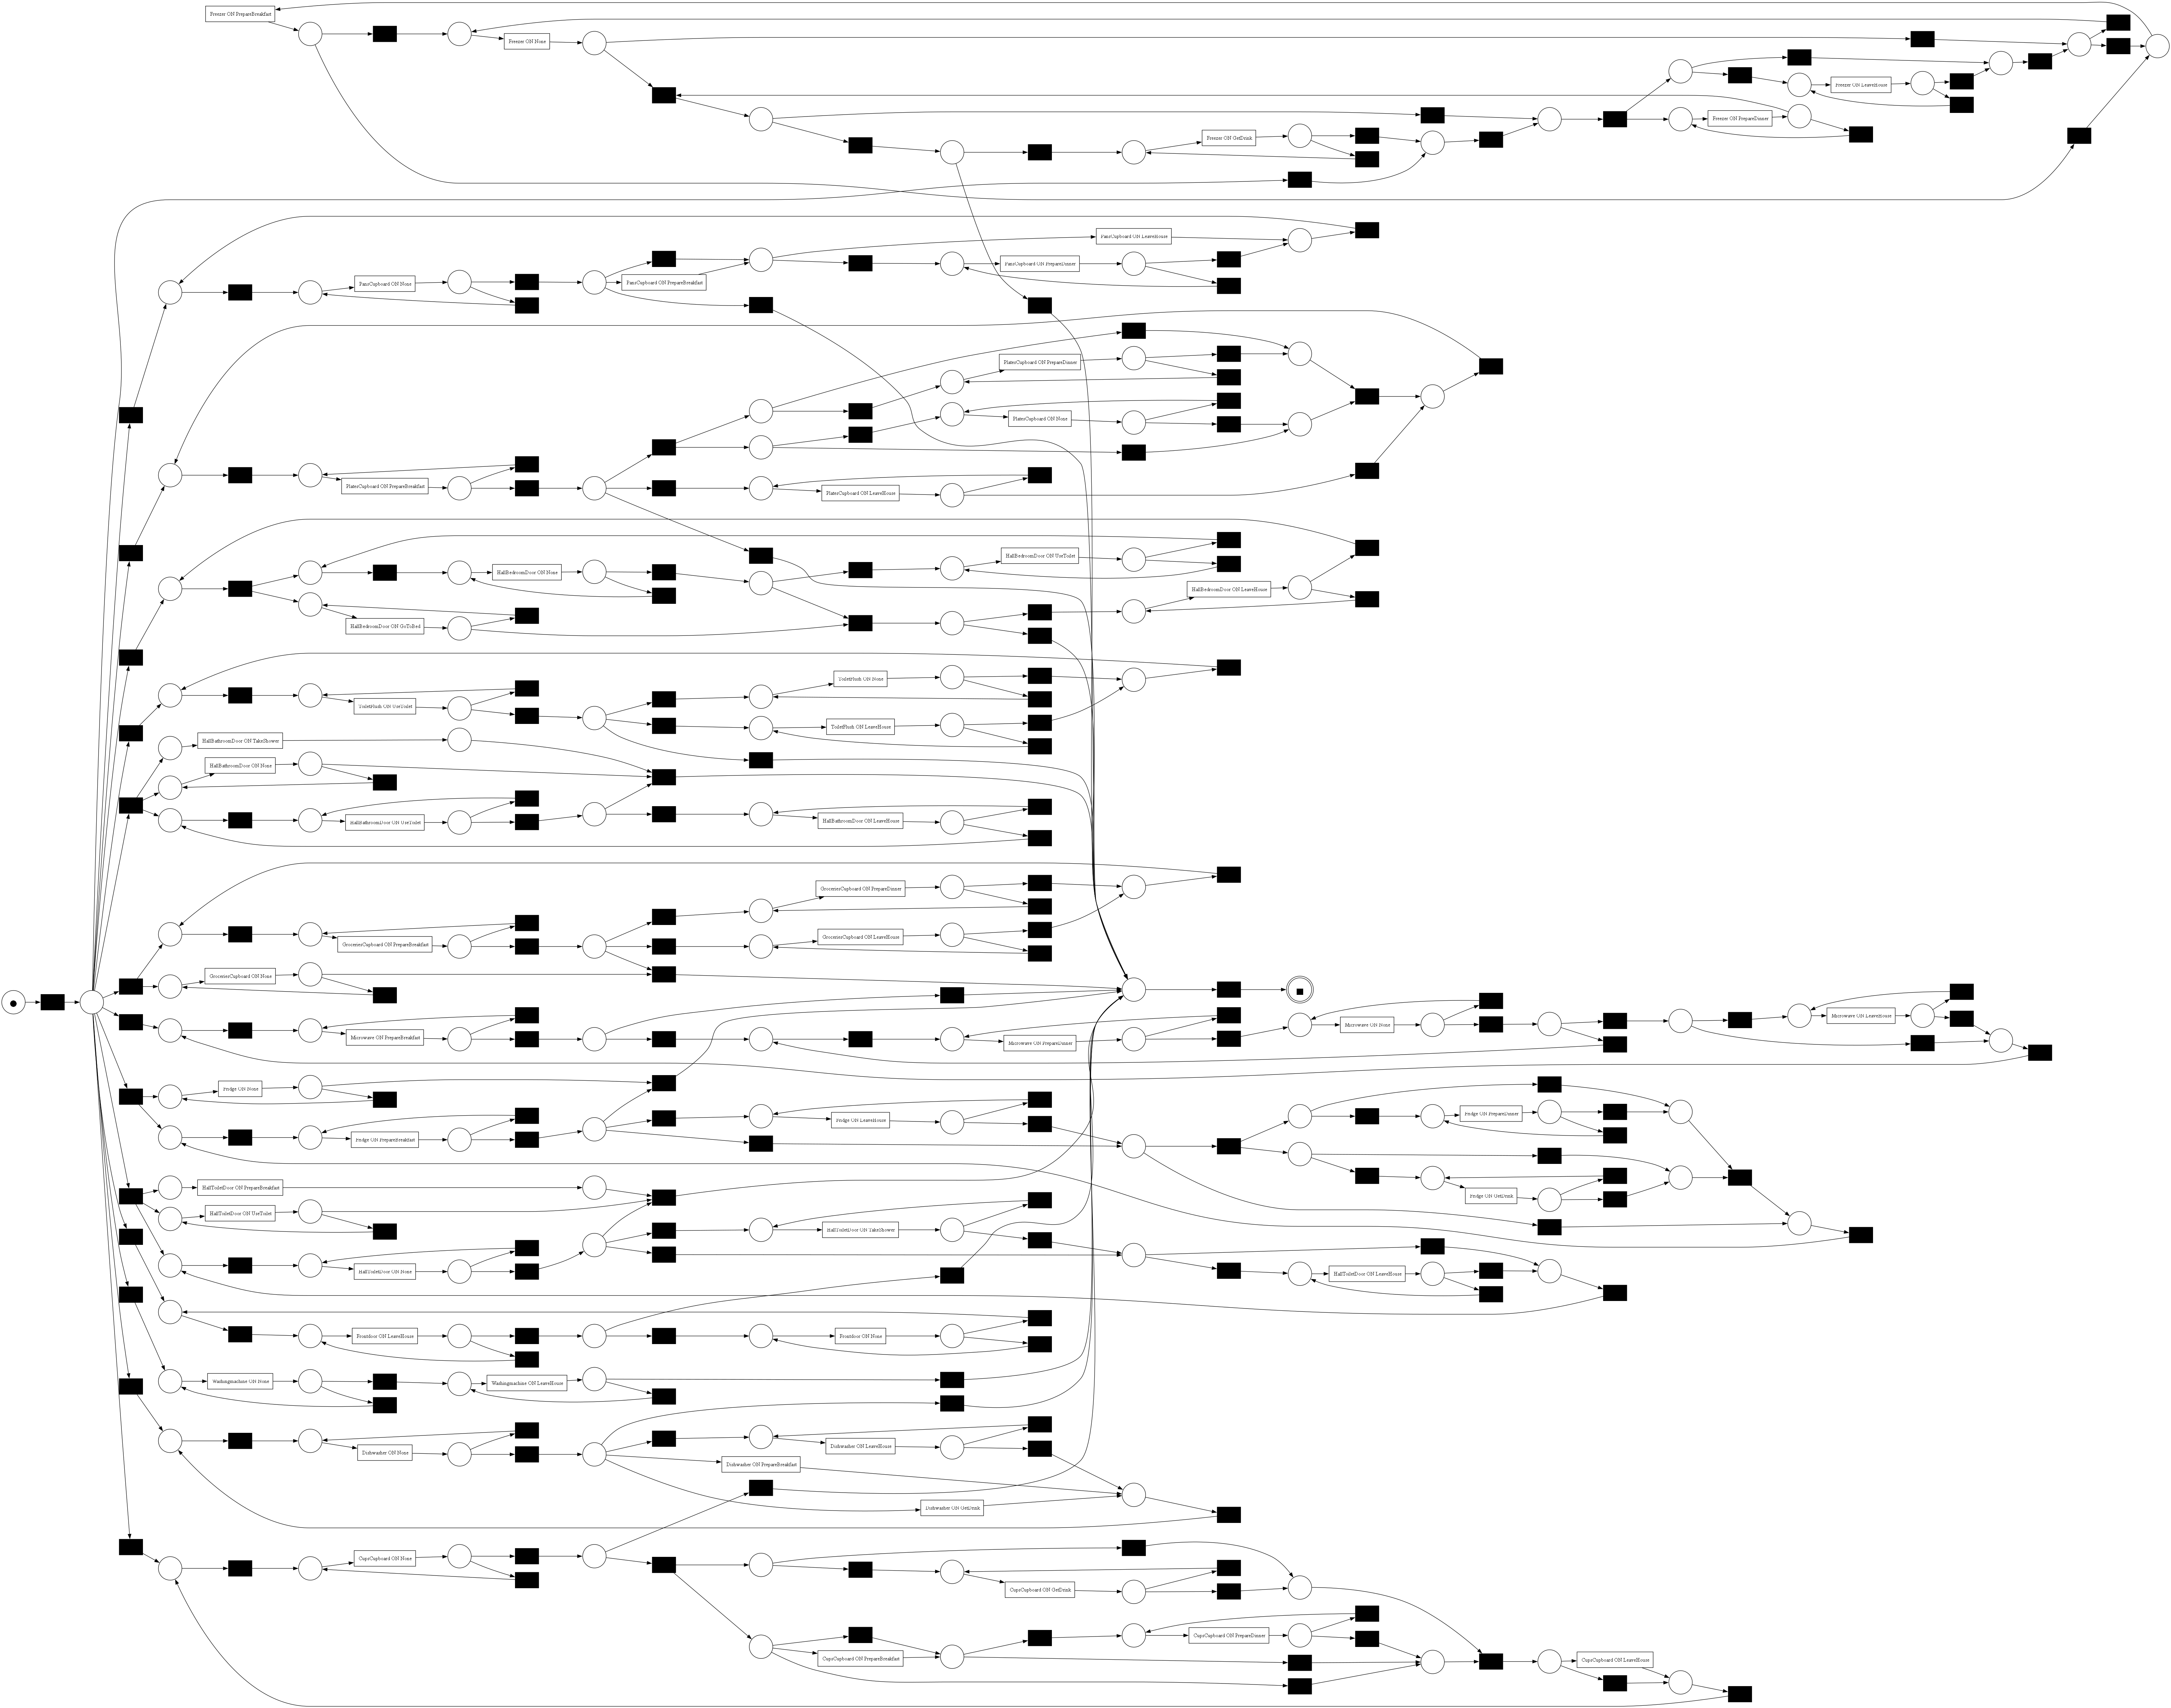
\includegraphics[width=\linewidth, height=\textheight]{images/inductive_minerGemini.png}
    \caption{Inductive Miner Petri Net}
\end{figure}



\begin{figure}[H]
    \centering
    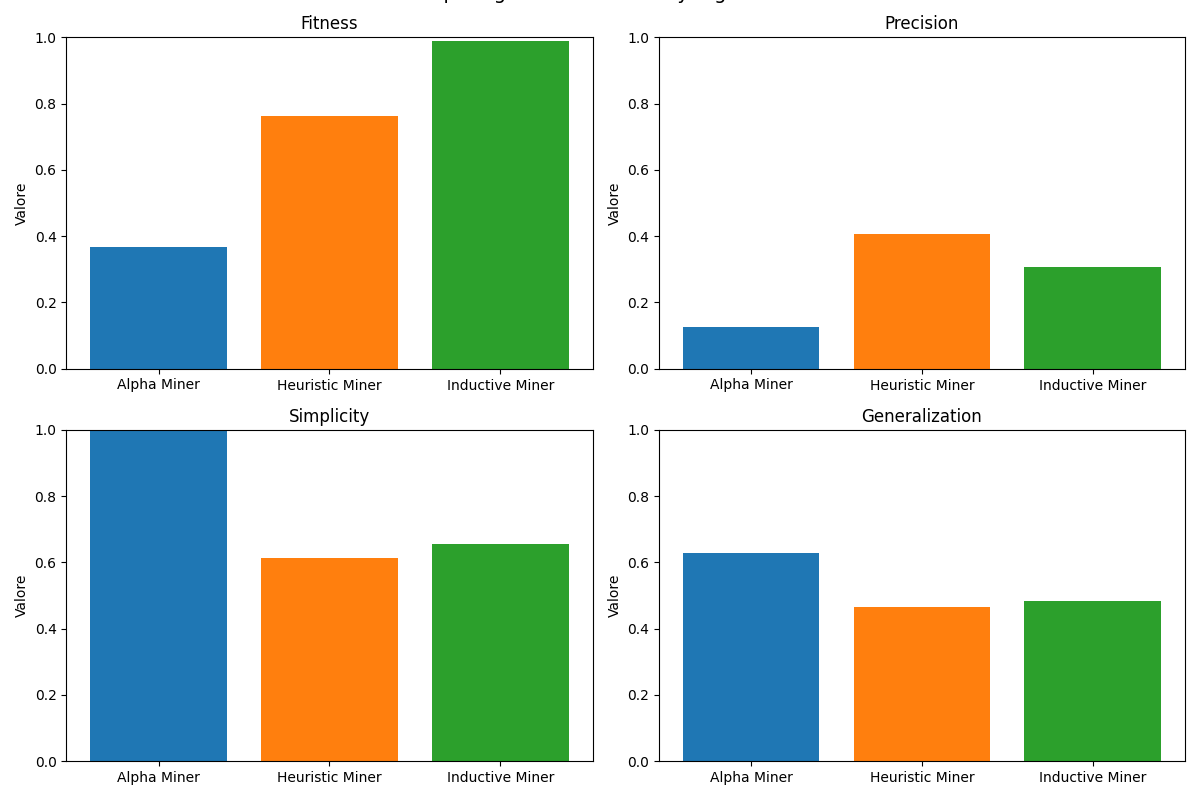
\includegraphics[scale=0.5]{images/metricsGemini.png}
    \caption{Performance metrics of the process mining algorithms}
\end{figure}


\begin{itemize}
    \item \textbf{Fitness:} Slightly reduced for all the algorithms
    \item \textbf{Precision:} Reduced for all the algorithms
    \item \textbf{Simplicity:} Same results
    \item \textbf{Generalization:} Same results
\end{itemize}

\subsubsection{Mistral}
The Mistral model returned 1314 new events. Basically, Mistral have duplicated the original dataset so the new events may not be consistent with the original dataset. The results are as follows:
\begin{figure}[H]
    \centering
    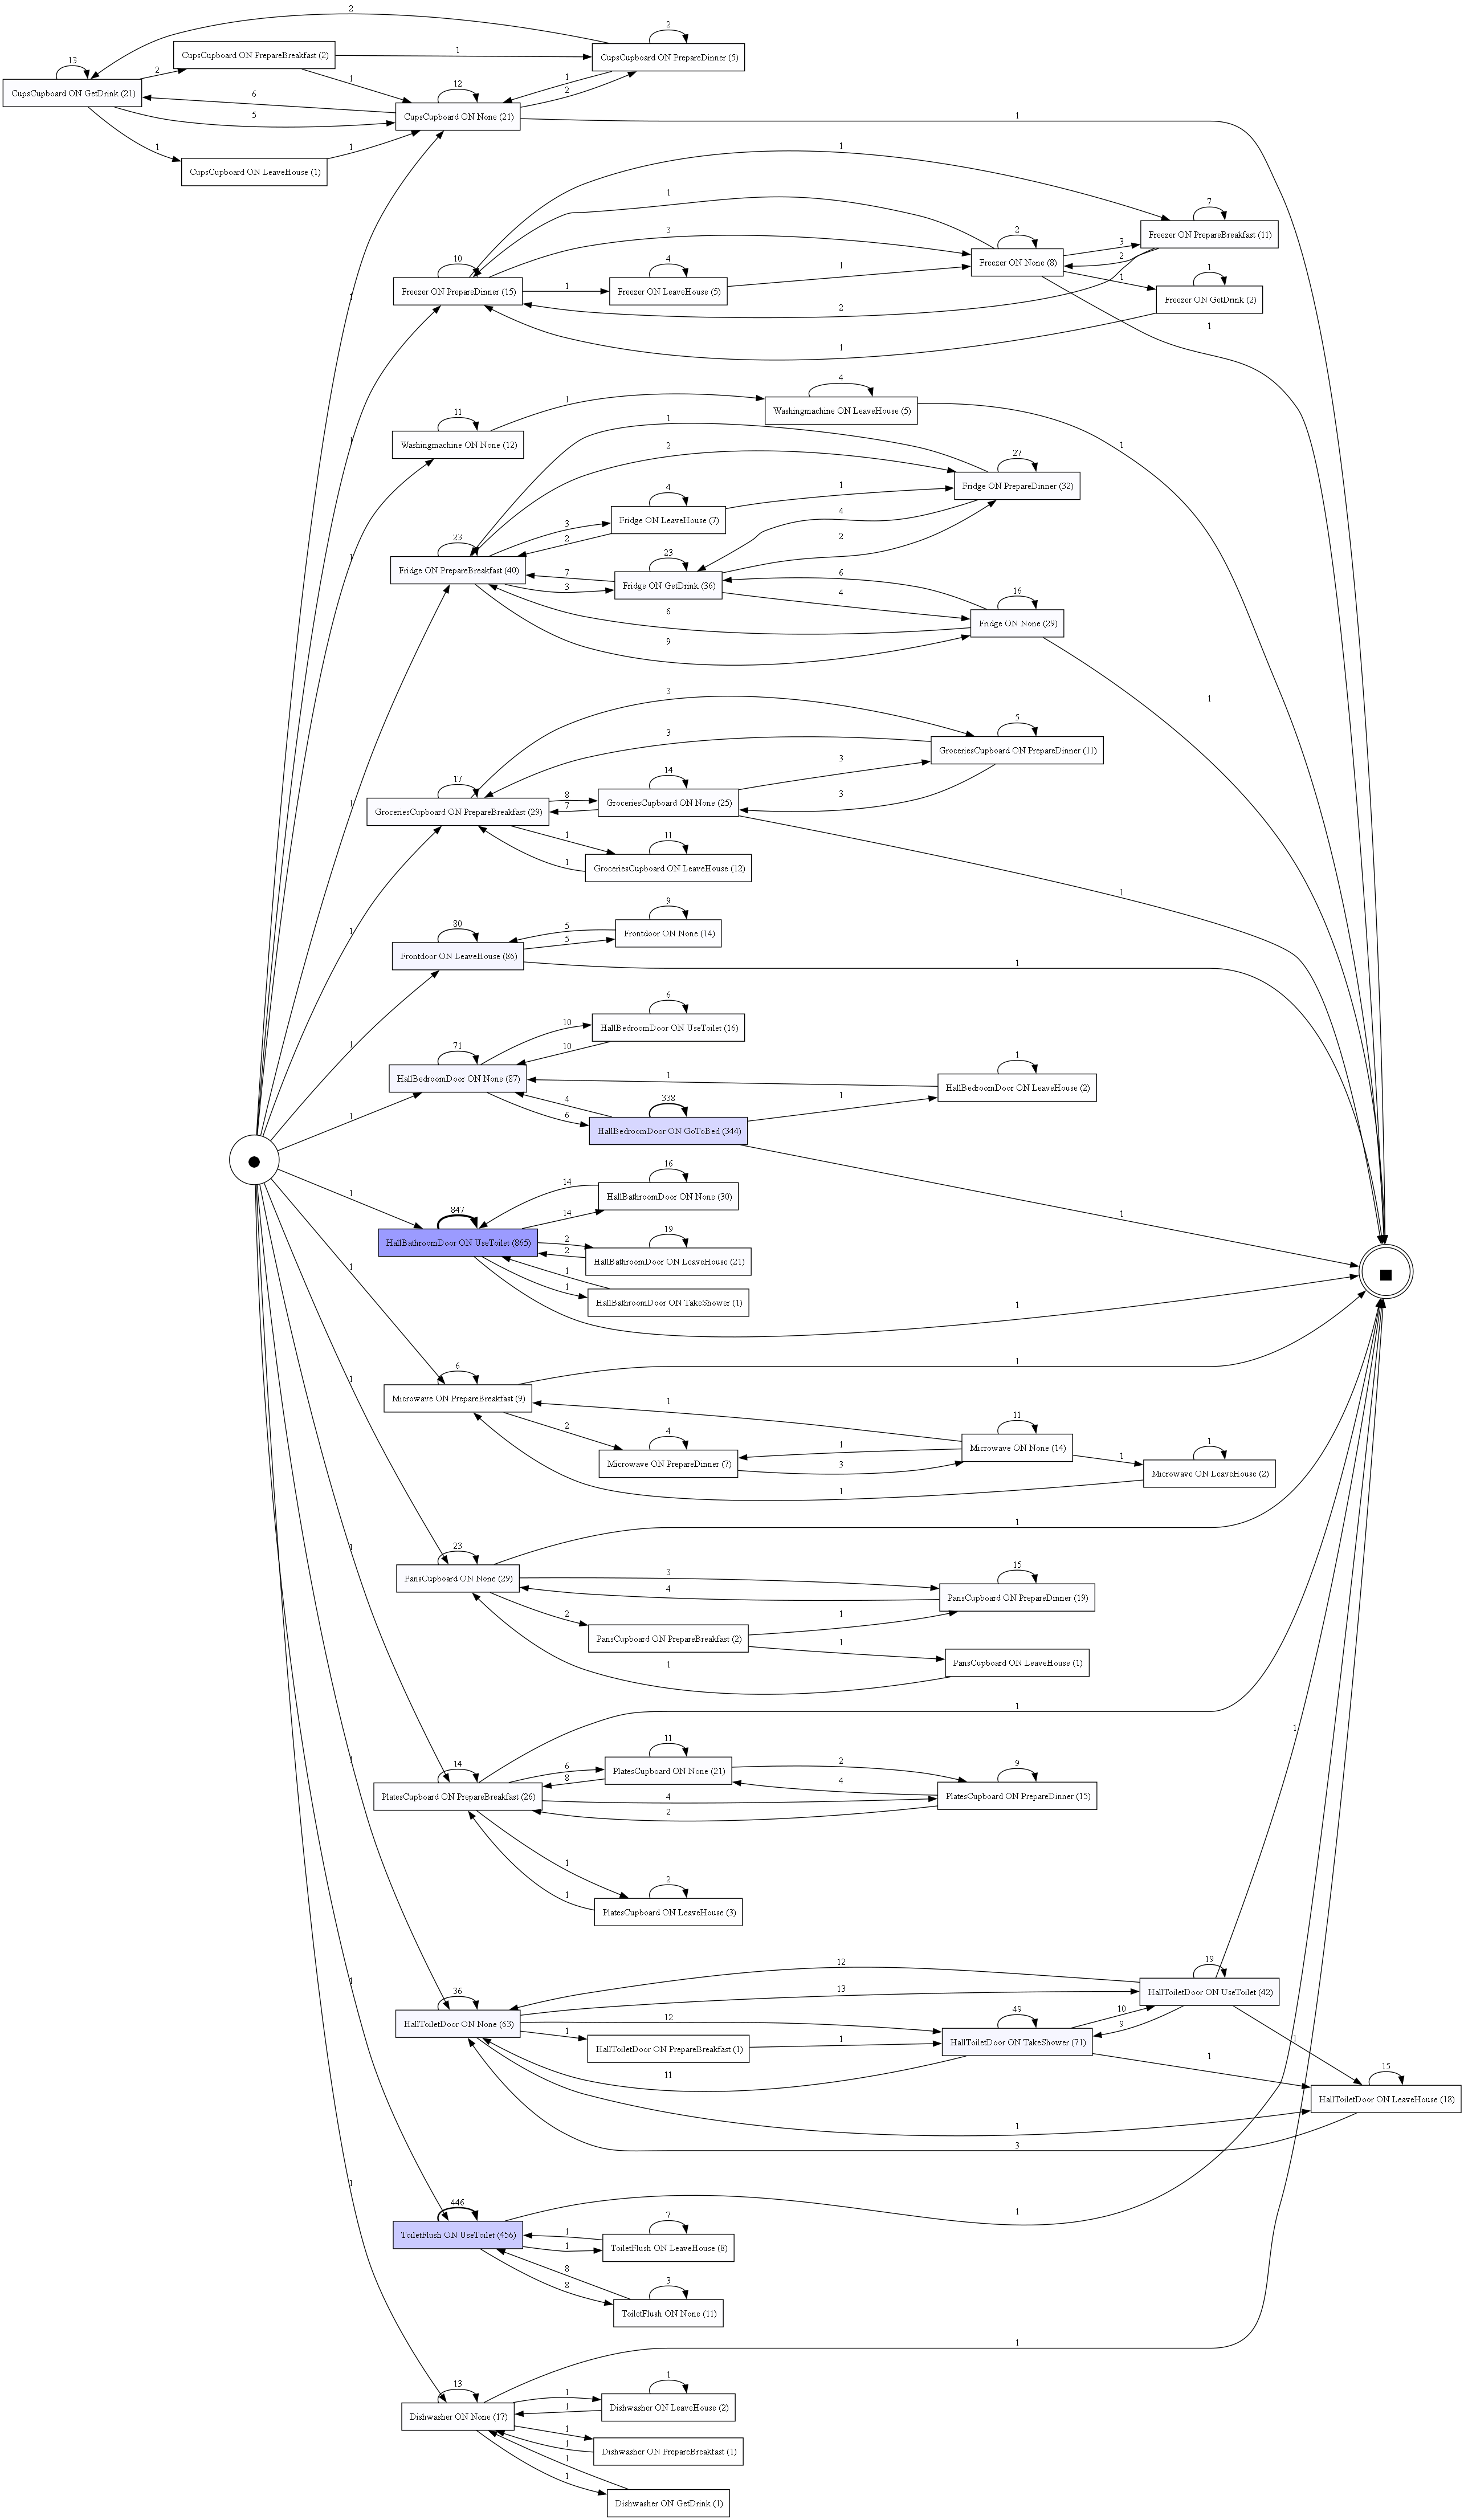
\includegraphics[width=\linewidth, height=\textheight]{images/dfgMistral.png}
    \caption{Directly-Follows Graph (DFG) of the event log}
\end{figure}

\begin{figure}[H]
    \centering
    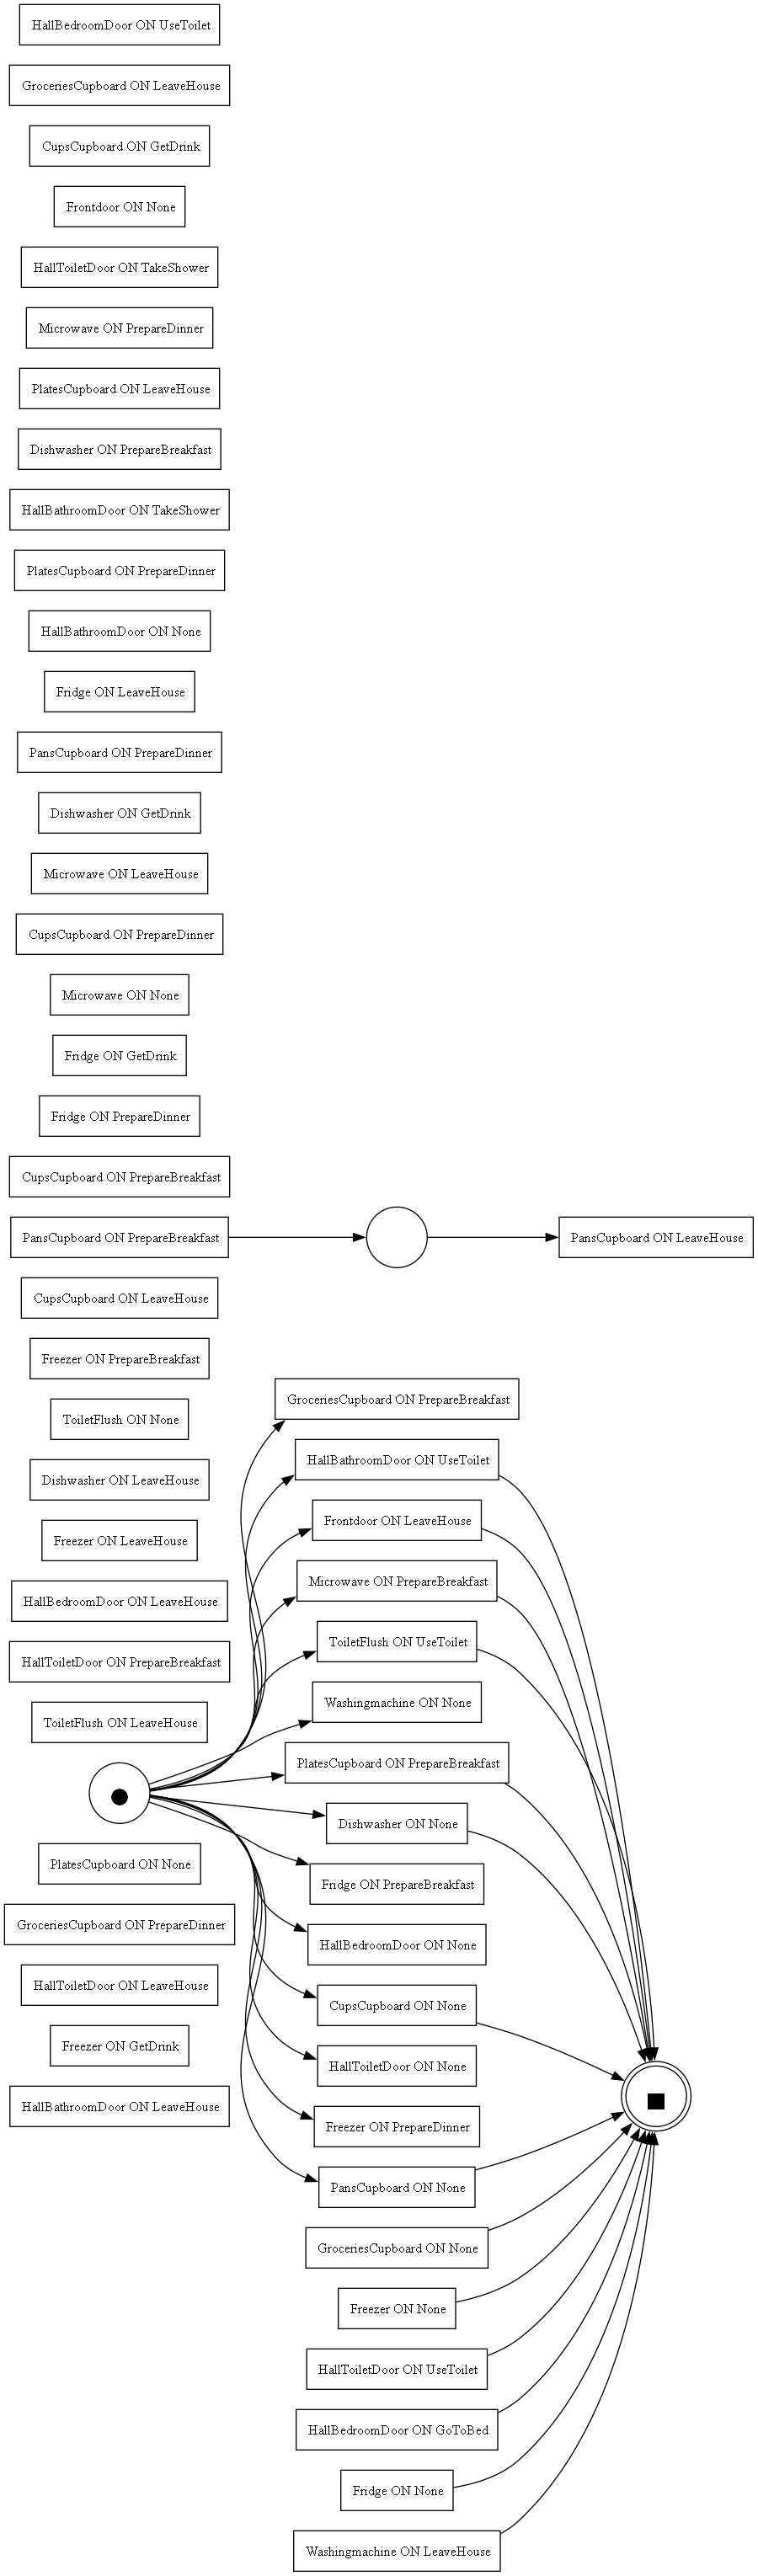
\includegraphics[width=\linewidth, height=\textheight]{images/alpha_minerMistral.png}
    \caption{Alpha Miner Petri Net}
\end{figure}

\begin{figure}[H]
    \centering
    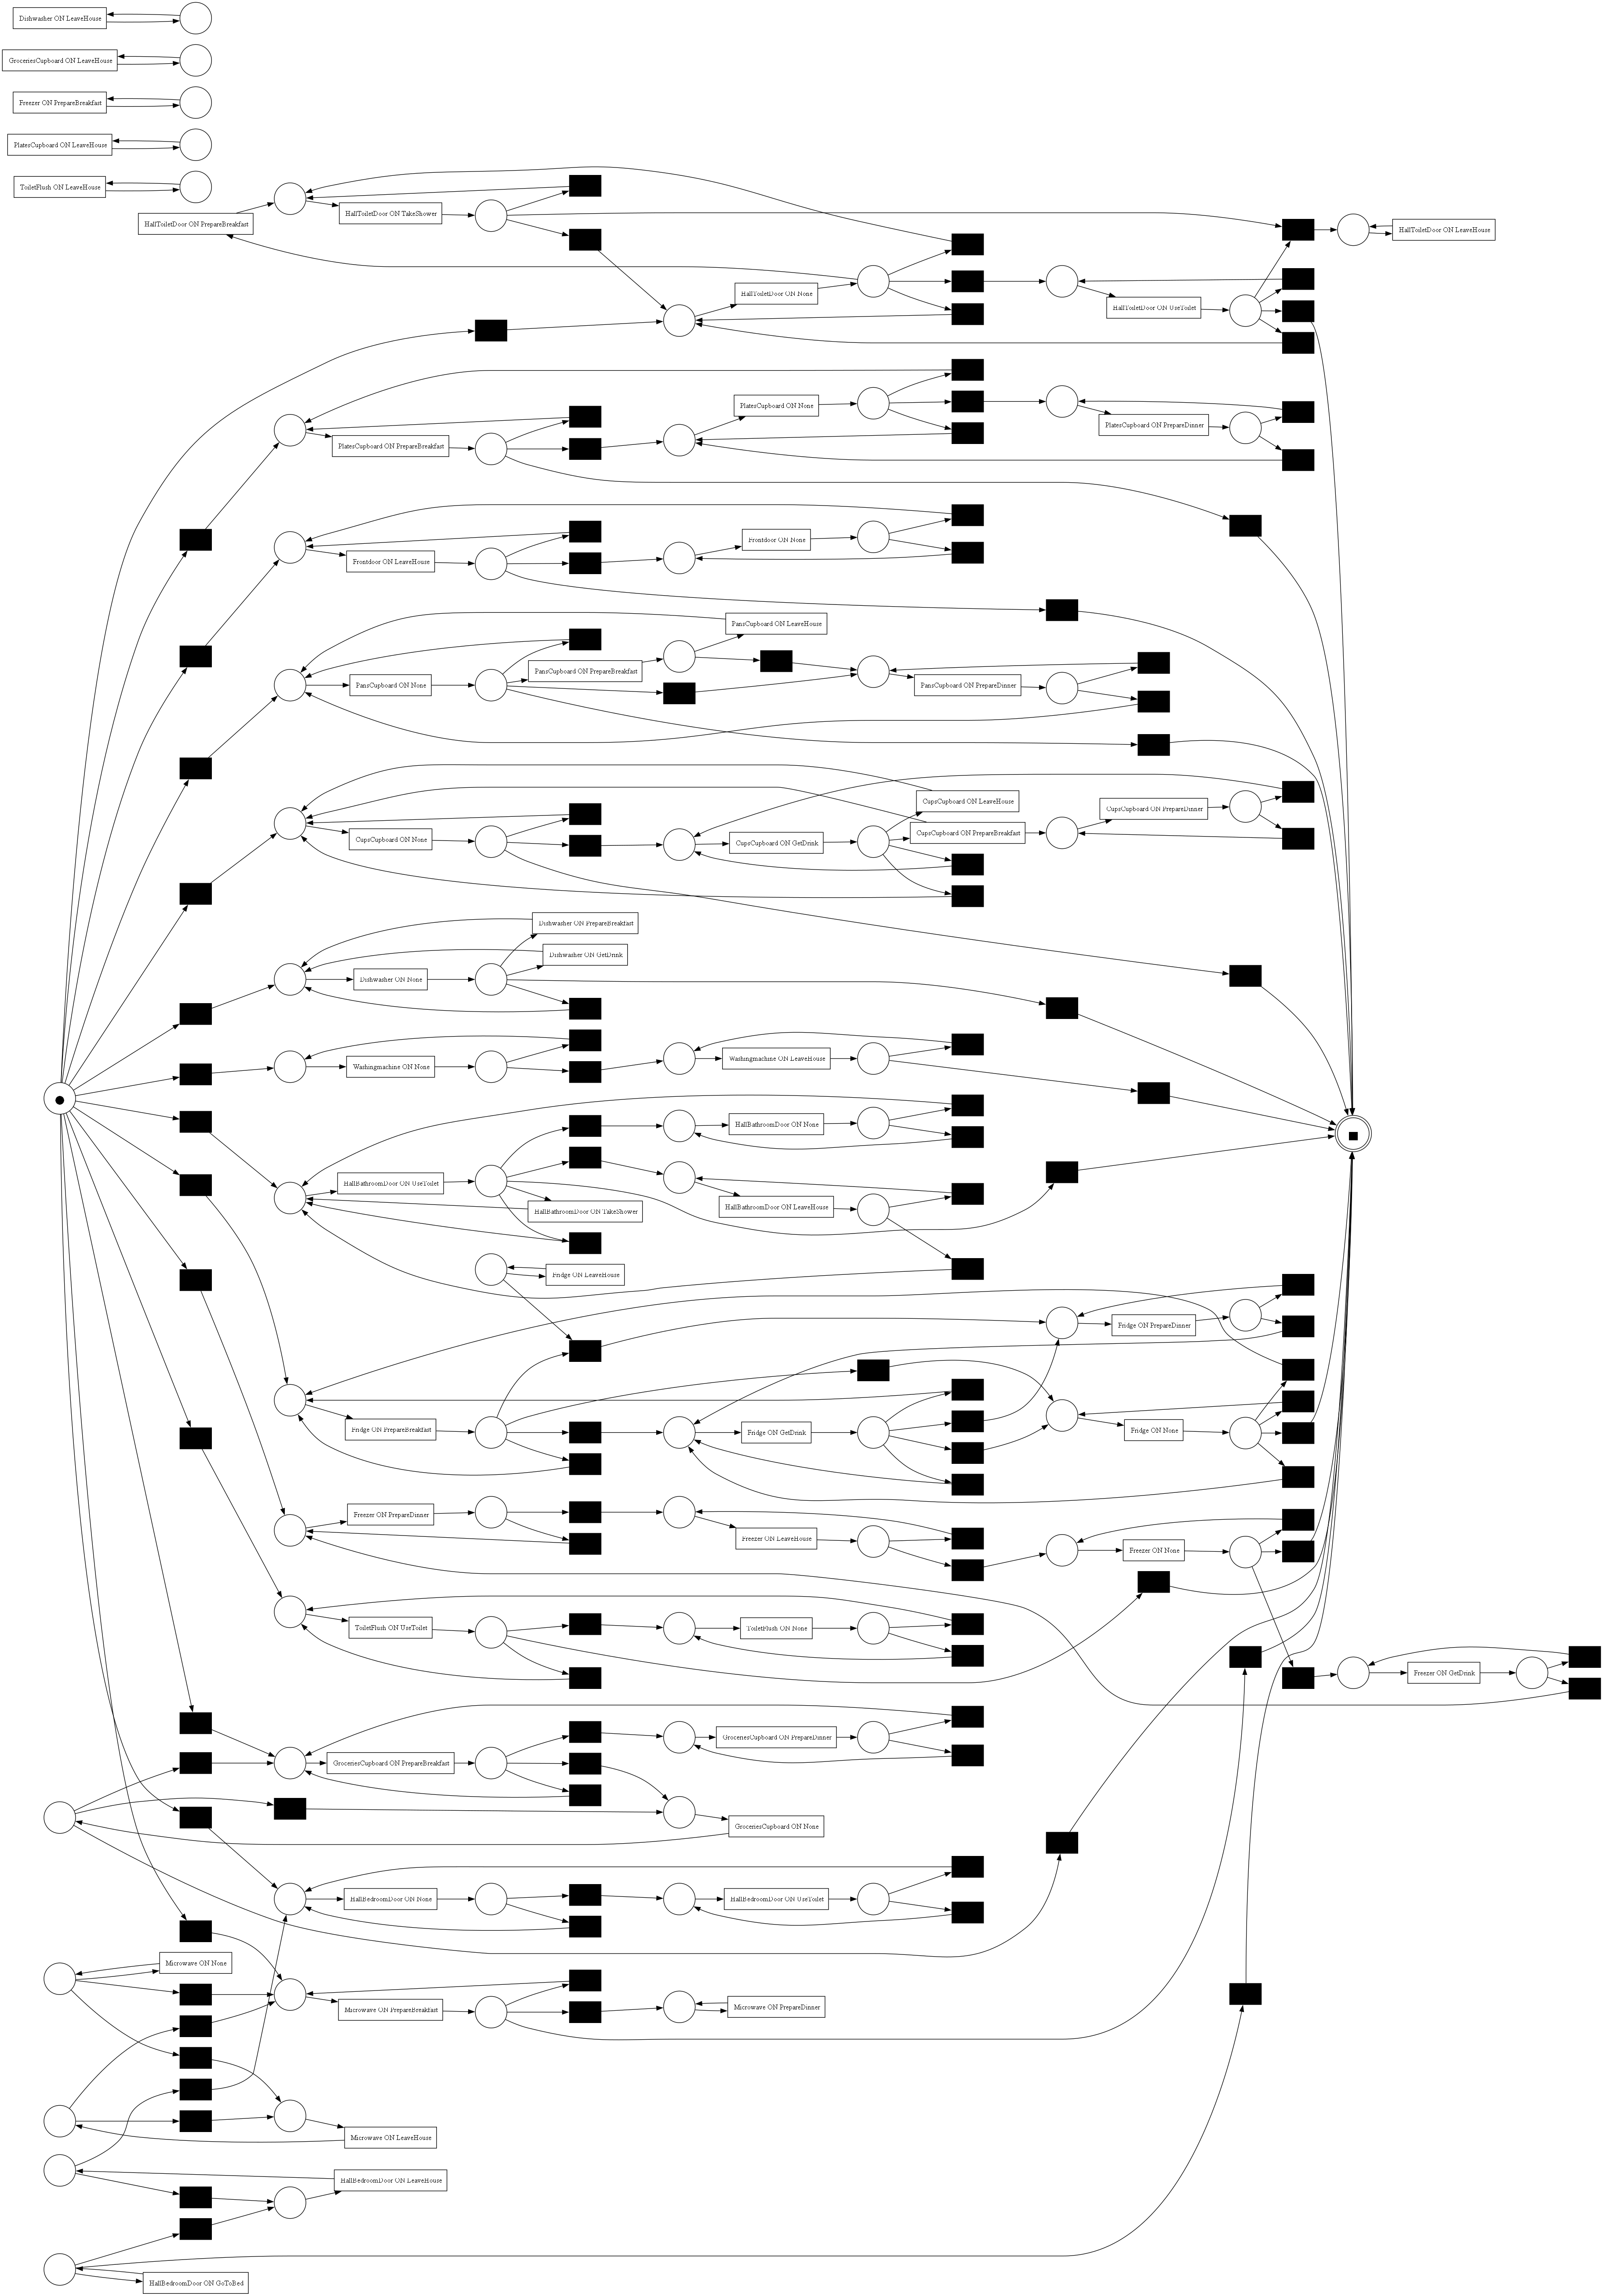
\includegraphics[width=\linewidth, height=\textheight]{images/heuristic_minerMistral.png}
    \caption{Heuristic Miner Petri Net}
\end{figure}

\begin{figure}[H]
    \centering
    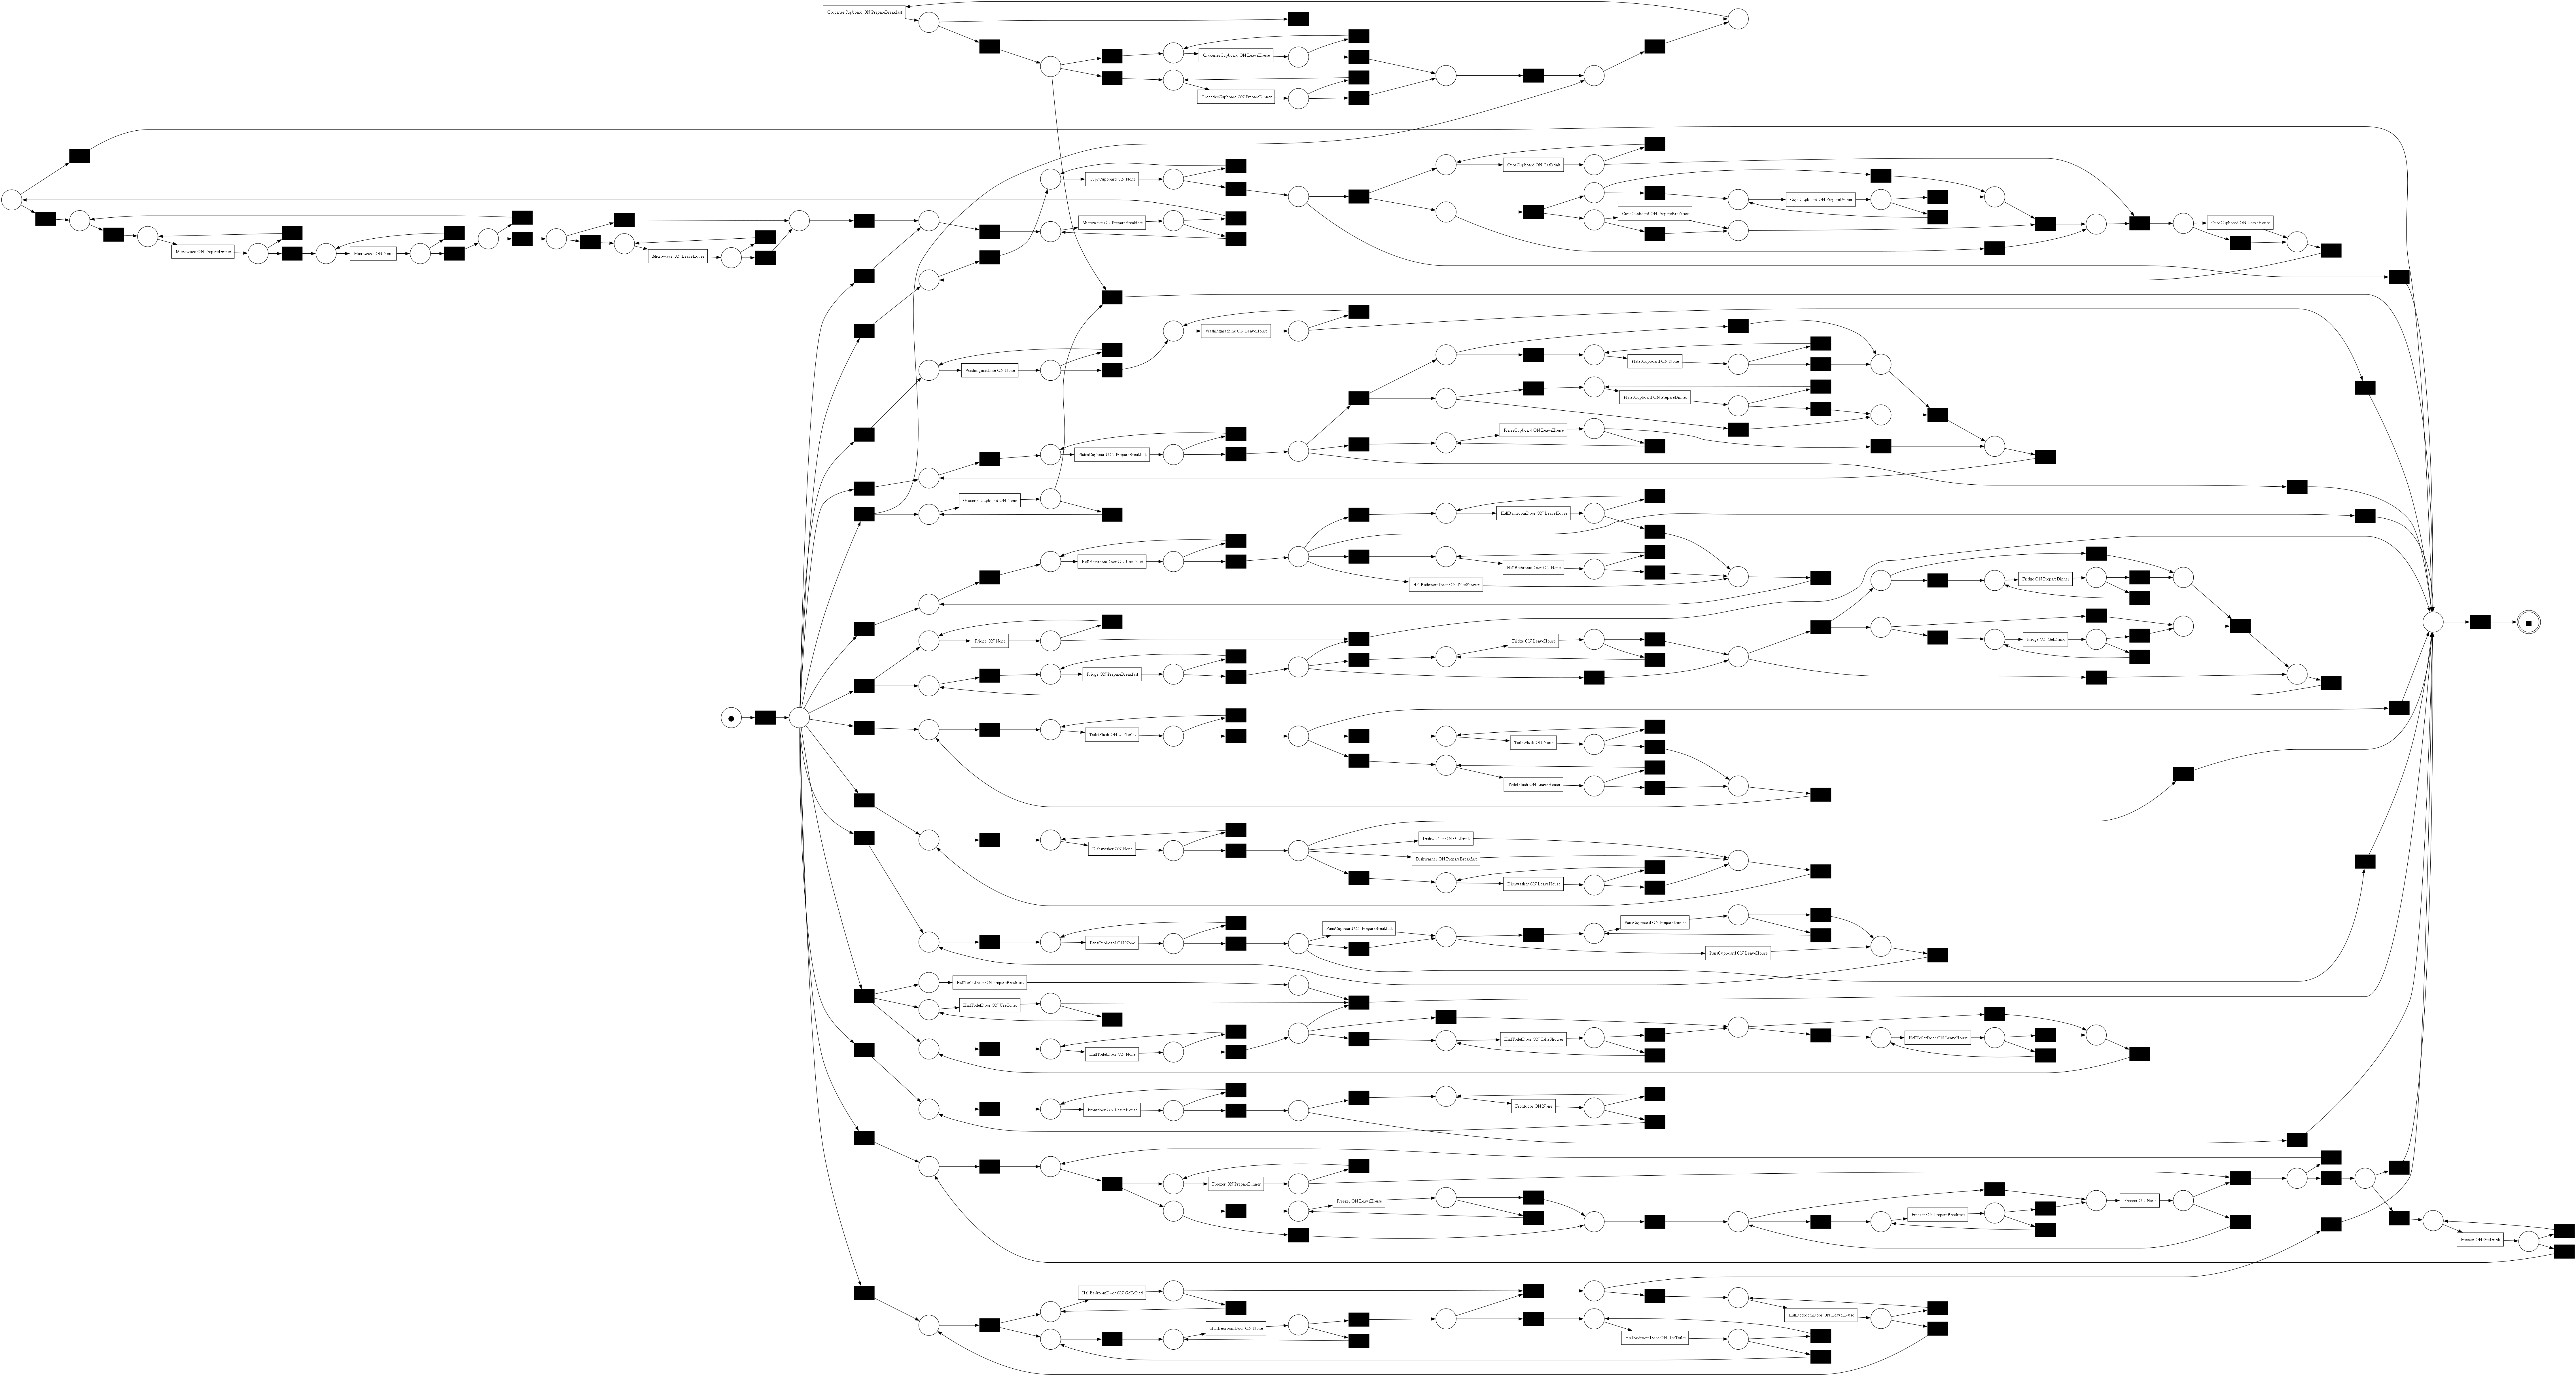
\includegraphics[width=\linewidth, height=\textheight]{images/inductive_minerMistral.png}
    \caption{Inductive Miner Petri Net}
\end{figure}

\begin{figure}[H]
    \centering
    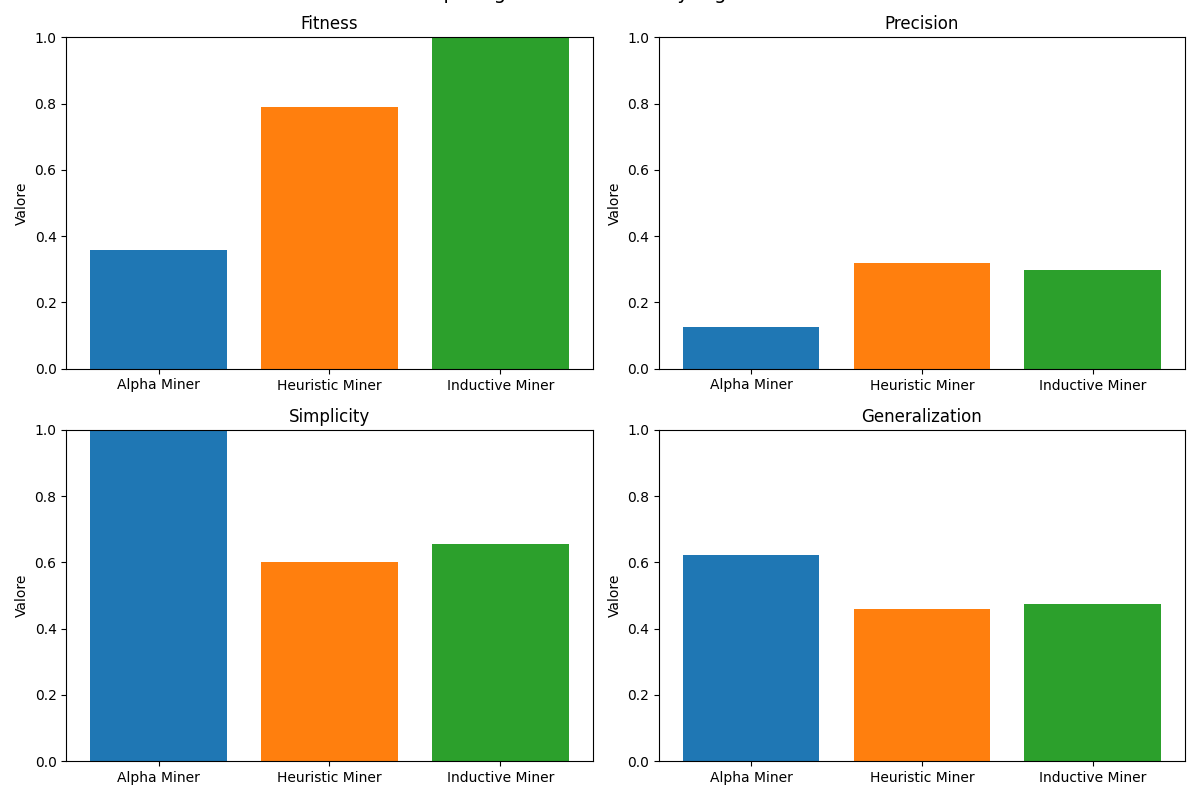
\includegraphics[scale=0.5]{images/metricsMistral.png}
    \caption{Performance metrics of the process mining algorithms}
\end{figure}


\begin{itemize}
    \item \textbf{Fitness:} Same results
    \item \textbf{Precision:} Slightly reduced for all the algorithms
    \item \textbf{Simplicity:} Same results
    \item \textbf{Generalization:} Same results
\end{itemize}

\subsection{Conclusion}

As we can see, all these experiments have reduced the performance of the process mining algorithms. The main reason for this is that the new events generated by the LLMs probably were not consistent with the original dataset or not so different. In the case of Mistral, the model simply duplicated the original dataset, which did not add any value to the process mining task. It could also depend on the original dataset, which was not so complex, and the LLMs struggled to generate new events that were consistent with the original dataset. In conclusion, the use of LLMs for data augmentation in process mining tasks is still an open research field, and further studies are needed to understand how to use these models effectively.
